\documentclass[a4paper, 12pt, parskip=half]{scrbook}

% Einfaches Copy and Paste ermöglichen
\usepackage{cmap}

% deutsche Silbentrennung
\usepackage[ngerman]{babel}

% deutsche Umlaute
\usepackage[utf8]{inputenc}
\usepackage[T1]{fontenc}

\usepackage{csquotes}

% Keine extra Leerzeichen nach einem Punkt
\frenchspacing

% Schriftart
\usepackage{times}

% Stichwortverzeichnis
\usepackage{imakeidx}
\makeindex

% Paket für Änderungen an Kopf- und Fußzeile
\usepackage{scrlayer-scrpage}
% Bisherige Einstellungen für Kopf- und Fußzeilen löschen:
\clearpairofpagestyles
% Einstellungen für die Fußzeile, die Kopfzeile wird nicht verwendet
	% Einstellungen nur für die rechten Seiten
	% Layout: |  Seite
\rofoot[\textbf{$\mid$~~\pagemark}]{\textbf{$\mid$~~\pagemark}}
	% Einstellungen nur für die linken Seiten
	% Layout: Seite  |
\lefoot[\textbf{\pagemark~~$\mid$}]{\textbf{\pagemark~~$\mid$}}

% Paket für code Beispiele
\usepackage{listings}

% Paket für Bilder
\usepackage{graphicx}
\graphicspath{ {./img/} }

% Paket für Verlinkungen
\PassOptionsToPackage{hyphens}{url}\usepackage[breaklinks]{hyperref}

\renewcommand{\UrlBreaks}{\do\/\do\-\do\_\do\&\do\?}	% allows URL breaking on /, -, _ and &

% Eigene Commands
\newcommand{\thesisTitle}{Entwurf und Realisierung eines Capture the Flag Core Systems}
\newcommand{\thesisTitleEnglish}{Design and implementation of a Capture the Flag Core System}
\newcommand{\thesisSubject}{CTF System für IT-Sicherheitsschulungen}
\newcommand{\thesisAuthor}{Robert Hartings}
\newcommand{\Matrikelnummer}{1164453}


% Literaturverzeichnis einrichten
\usepackage[style=alphabetic, citestyle=alphabetic]{biblatex}
\addbibresource{thesis.bib}

\hypersetup{
	unicode = true, % allows to use characters of non-Latin based languages in Acrobat’s bookmarks 
	pdftitle = {\thesisTitle}, % define the title that gets displayed in the "Document Info" window of Acrobat 
	pdfauthor = {\thesisAuthor},
	pdfsubject = {\thesisSubject},
	pdfkeywords = {ITS2, hack-me-if-you-can},
	colorlinks = true,
	citecolor = black,
	filecolor = black,
	linkcolor = black,
	urlcolor = black,
	linktoc = all,
}

\title{\thesisTitle}
\author{\thesisAuthor}
\date{\today{}}

\begin{document}
	% Vorspann einleiten:
	\frontmatter
	
	\begin{titlepage}
	
\begin{center}
		\textbf{\Large Entwurf und Realisierung eines}\\
		\textbf{\Large Capture the Flag Core Systems}\\[3cm]
		\textbf{Bachelorarbeit}\\
		zur Erlangung des Grades {\em Bachelor of Science}\\[1.5cm]
		
		an der\\
		Hochschule Niederrhein\\
		Fachbereich Elektrotechnik und Informatik\\
		Studiengang {\em Informatik}\\[3cm]
		
		vorgelegt von\\
		\thesisAuthor\\
		Matrikelnummer: \Matrikelnummer\\[3cm]
		Datum: 4. August 2020\\[3cm]
		
		Prüfer:~Prof.~Dr.~Jürgen Quade\\
		Zweitprüfer:~Prof.~Dr.~Peter~Davids
	\end{center}
\end{titlepage}
	\cleardoublepage
	\pagestyle{scrheadings}
	%-------------------------------------
\section*{Eidesstattliche Erklärung}
%-------------------------------------

\begin{tabbing}
	Matrikelnummer: \= \kill
	Name: \> \thesisAuthor\\
	Matrikelnr.: \> \Matrikelnummer\\
	Titel: \> \thesisTitle\\
	Englischer Titel: \> \thesisTitleEnglish\\
\end{tabbing}

Ich versichere durch meine Unterschrift, dass die vorliegende Arbeit ausschließlich von mir verfasst wurde.
Es wurden keine anderen als die von mir angegebenen Quellen und Hilfsmittel benutzt.

Die Arbeit besteht aus \underline{\hspace{3em}} Seiten.

\vspace{6ex}
\begin{tabbing}
\underline{\hspace{14em}} \hspace{3em}\= \underline{\hspace{14em}} \\
Ort, Datum \> \thesisAuthor
\end{tabbing}
	\tableofcontents	

	
	% Hauptteil einleiten:
	\mainmatter
	
	% Einstellungen für die Fußzeile aktualisieren
		% Einstellungen nur für die rechten Seiten
		% Layout: Abschnitt  |  Seite
	\rofoot[\textbf{\headmark~~$\mid$~~\pagemark}]{\textbf{\headmark~~$\mid$~~\pagemark}}
		% Einstellungen nur für die linken Seiten
		% Layout: Seite  |  Kapitel
	\lefoot[\textbf{\pagemark~~$\mid$~~Kapitel~\headmark}]{\textbf{\pagemark~~$\mid$~~Kapitel~\headmark}}
	
	\chapter{Einleitung}
	\label{chap:Einleitung}
	\label{chap_text:Einleitung}
Das Thema IT Sicherheit ist besonders in den letzten Jahren relevant geworden. Viele Firmen suchen Fachkundige \cite{it-daily.netITSecurityExpertenWerdenHanderingend2019}, die die bestehenden und neu designten Systeme und Programme auf Sicherheitslücken prüfen und Lösungsvorschläge zu deren Behebung präsentieren. Auch werden Experten gesucht, die die im Unternehmen bestehenden Prozesse prüfen und neue zum Umgang mit Sicherheitslücken entwerfen.

Einen Mangel an IT-Sicherheit in privaten und öffentlichen Unternehmen, beziehungsweise ein fehlendes Konzept zur Vorbeugung, Erkennung und Abwendung von Sicherheitslücken sieht man in jüngster Vergangenheit deutlich, nachdem beispielsweise diverse Universitäten wie Gießen \cite{schirmacherUniGiessenNaehert2020}, Maastricht \cite{wdrCyberattackeHackerangriffAuf2019} und Bochum \cite{ruhr24HackerAngriffLegtITSysteme2020} Ende 2019 Ziele von Hackerangriffen geworden sind. Aber nicht nur Universitäten sind betroffen, so sind neben Gerichten \cite{hurtzHackerAngriffAufGericht2020}, Stadtverwaltungen \cite{barsigCyberAttackeAufPotsdamer2020} und Krankenhäusern \cite{wellbrockITSicherheitImKrankenhaus2019} bereits der Deutsche Bundestag von Hackern angegriffen und kompromittiert worden. \cite{fladeCyberangriffAufBundestag2020}

In der Studie \textquote{Wirtschaftsschutz in der digitalen Welt} vom 06. November 2019 des Bundesverbandes Informationswirtschaft, Telekommunikation und neue Medien e.V. Bitkom wird die aktuelle Bedrohungslage durch Spionage und Sabotage für deutsche Unternehmen untersucht. Daraus geht hervor, dass im Jahr 2019 von Datendiebstahl, Industriespionage oder Sabotage 75\% der befragten Unternehmen\footnote{Die Grundlage der Studie sind 1070 (2019) und 1074 (2015) befragte Unternehmen} betroffen  und 13\% vermutlich betroffen waren. Die Zahlen dieser Unternehmen ist steigend. Im Jahre 2015 waren \textquote{nur} 51\% betroffen und 28\% vermutlich betroffen. Die Unternehmen beziffern den Schaden auf 102,9 Milliarden Euro pro Jahr. \cite{bergWirtschaftsschutzDigitalenWelt2019}

Dass diese Thematik auch im Lehrbetrieb angekommen ist, sieht man an neu startenden Studiengängen wie dem Bachelorstudiengang Cyber Security Management der Hochschule Niederrhein, der zum Wintersemester 2020/21 startet. \cite{hochschuleniederrheinHackernRoteKarte2020}

Es ist zu erwähnen, dass die Hochschulen sich bereits mit dem Thema auseinandersetzen. 
So beschäftigt sich an der Hochschule Niederrhein das Institut für Informationssicherheit Clavis besonders mit Themen rund um das Informationssicherheitsmanagement, gestaltet aber auch Inhalte zur Vulnerabilität von (kritischer) Infrastruktur und Hacking.
Das Ziel von Clavis ist die Erhöhung der Informationssicherheit von Organisationen im regionalen Umfeld der Hochschule.
\cite{hochschuleniederrheinFlyerInstitutClavis}
Auch hat die Hochschule Niederrhein das Thema IT-Sicherheit bereits in ihren Lehrplan für die Studiengänge Informatik und Elektrotechnik am Fachbereich 03 Elektrotechnik und Informatik aufgenommen. So werden dort im fünften Semester in der Veranstaltung IT-Security grundlegende Kompetenzen zum Thema IT-Sicherheit vermittelt, welche einem allgemeinen Anspruch genügen. \cite{hochschuleniederrheinModulhandbuchVollzeitBA2019}

Begleitend zu dieser Veranstaltung werden drei Versuche im Rahmen des Praktikums durchgeführt. Diese sollen den Studierenden praktische Erfahrungen ermöglichen und ein breites Bewusstsein schaffen, indem die Studierenden sowohl in die Rolle des Angreifers als auch die des Verteidigers schlüpfen.

Im zweiten Versuch namens \textquote{Catch me, if you can} findet ein Vergleichswettbewerb zwischen den teilnehmenden Studierendenteams statt.

Die Aufgabe der Teams besteht darin, festgelegte Programme/Dienste abgesichert bereit zustellen, geheime Informationen sowohl auf dem eigenen Rechner als auch auf den Rechnern der anderen Teams zu finden und Schwachstellen abzusichern, um so zu verhindern, dass andere Teams an die eigenen geheimen Informationen gelangen. \cite[S. 2]{sosnaKonzeptionUndRealisierung2010} 

Die geheimen Informationen sind normalerweise Passwörter oder private Bilder und werden im Versuch durch sogenannte Flags repräsentiert. Eine Flag ist eine generierte Zeichenfolge mit fester Länge.
	\section{Motivation}
\label{sec:Motivation}
Neben diversen Meldungen zu erfolgreichen Angriffen auf Unternehmen und öffentliche Körperschaften und durch die Veranstaltung IT-Sicherheit im fünften Semester, besonders herauszuheben ist hier das Praktikum\footnote{Praktikum ist hierbei mit einer Pflichtübung vergleichbar}, bin ich auf das Thema IT-Sicherheit aufmerksam geworden. 

Die zunehmenden Vorfälle zeigen, dass ein breites Bewusstsein für IT-Sicherheit geschaffen werden muss.

Der Versuch \textquote{Catch me, if you can} versucht dieses Bewusstsein zu schaffen, in dem die Studierenden sowohl in die Rolle des Angreifers als auch die des Schützers schlüpfen.

Das Programm, welches das Praktikum überwacht, ist bereits 10 Jahre alt und bietet meiner Meinung nach Notwendigkeiten der Modernisierung, Überarbeitung und Erweiterung. 
So gibt es beispielsweise heute bessere Möglichkeiten die Darstellung (Web-Oberfläche) zu realisieren.
	\section{Aufgabenstellung}
\label{sec:Aufgabenstellung}
Begleitend zu der Veranstaltung IT-Security für die Studiengänge Bachelor Informatik und den Bachelor Elektrotechnik des Fachbereichs 03 Elektrotechnik und Informatik der Hochschule Niederrhein werden 3 Praktika durchgeführt. Diese sollen den Studierenden praktisch Erfahrungen ermöglichen.

Das zweite Praktikum \textquote{Catch me, if you can} stellt einen Vergleichswettbewerb dar. An diesem Wettbewerb nehmen mehrere Teams teil, welche sich alle in einem gemeinsamen Netzwerk befinden. Die Aufgabe der Teams besteht darin, festgelegte IT-Dienste (abgesichert) bereit zustellen, geheime Informationen sowohl auf dem eigenen Rechner als auch auf den Rechnern der anderen Teams zu finden und zu verhindern, dass andere Teams an die eigenen geheimen Informationen gelangen.\cite[S. 2]{sosnaKonzeptionUndRealisierung2010} Die geheimen Informationen sind logisch gesehen Passwörter oder private Bilder und werden durch sogenannte Flags repräsentiert. Eine Flag ist ein gehashter Zeichenfolge und hat immer die gleiche Länge.

Das Praktikum wird durch ein Auswertungs- und Überwachungssystem überwacht - anderes Wort -, welches eine objektiv nachvollziehbare Bewertung vornehmen kann und die in den Bewertungsprozess eingeflossenen Parameter dokumentiert.\cite[S. 2]{sosnaKonzeptionUndRealisierung2010}

Ziel meiner Arbeit ist die Modernisierung und Verbesserung dieses Auswertungs- und Überwachungssystems.

In der einführenden Betrachtung (\autoref{chap:Analyse}) wird der aktuelle Stand des Systems, Schnittstellen zwischen Server und Client sowie der Begründung für die Veränderung dargelegt. 

Aus dieser einführenden Betrachtung werden dann im \autoref{chap:Entwurf} Entwurf Anforderungen abgeleitet und Entwürfe für die verschieden Komponenten des Servers erstellt. 

An Hand der abgeleiteten Anforderungen und des Entwurfs der verschiedenen Komponenten wird im \autoref{chap:Technologien} Technologien verschiedene Technologien diskutiert und passende Technologien ausgewählt.

Die Implementierung des Entwurfs mit den gewählten Technologien wird im \autoref{chap:Realisierung} Realisierung beschrieben.

Eine kritische Auseinandersetzung mit dem Ergebnis dieser Arbeit folgt und es werden Aussichten für mögliche Veränderungen und Verbesserungen gegeben.
	
	\chapter{Analyse}
	\label{chap:Analyse}
	\label{chap_text:Analyse}
In diesem Kapitel werden die Voraussetzungen im Labor vorgestellt, die derzeitige Implementierung des Auswertungs- und Überwachungssystems beleuchtet und kurz auf einen überwachten Client sowie dessen Schnittstellen zum System eingegangen.
	\section{Lehrveranstaltung IT-Sicherheit} \label{sec:Lehrveranstaltung_IT-Sicherheit}

Das Pflichtmodul IT-Sicherheit (ITS) ist in drei Veranstaltungen gegliedert.\cite[S.30]{hochschuleniederrheinModulhandbuchVollzeitBA2019}
\begin{itemize}
	\item Vorlesung (2 Semesterwochenstunden)
	\item Übung (1 Semesterwochenstunde)
	\item Praktikum (1 Semesterwochenstunde)
\end{itemize}

\subsubsection{Vorlesung}
Die Vorlesung wird im wöchentlichen Turnus angeboten und behandelt grundlegendes Wissen zur IT-Sicherheit unter anderem in den Bereichen Gefährdung, Gegenmaßnahmen, aber auch im Bereich rechtliche Gegebenheiten. Es werden Beispiele aufgezeigt, bei denen die angesprochenen Themen gar nicht oder in einem ungenügenden Zustand umgesetzt worden sind. Die Vorlesung wird von den Veranstaltungen \textit{Übung} (freiwillig) und \textit{Praktikum} (verbindlich) ergänzt.

\subsubsection{Übung}
Die Übungen sind freiwillig und werden im zweiwöchentlichen Turnus á 2 Stunden angeboten. Diese ermöglichen es den Studierenden, den durch die Vorlesung und das Selbststudium vermittelten Stoff zu vertiefen und zu festigen. Auch können dort praktische Erfahrungen gesammelt werden, von denen die Studierenden unter anderem im Praktikum profitieren können.

\subsubsection{Praktikum}
Das Praktikum findet im monatlichen Turnus (3x im Semester á 4 Stunden) statt. Es ist in drei Laborversuche untergliedert. Nach Bestehen aller Versuche erhalten die Studierenden ihre Klausurzulassung. Jeder Versuch des Praktikums muss vorbereitet werden, dazu erhalten die Studierenden vor dem Versuch ein Hackit\footnote{Knobelaufgabe aus dem Bereich IT-Sicherheit / Hacking}. Nur mit erfolgreichem Absolvieren des Hackits ist es möglich, am nächsten Versuch teilzunehmen.\cite{quadePraktikumITSecurity2017}
	\section{Ausstattung Labor}
\label{sec:Ausstattung_Labor}

Das Praktikum wird im Labor für Echtzeitsysteme (EZS Labor) der Hochschule Niederrhein durchgeführt.

\begin{center}
	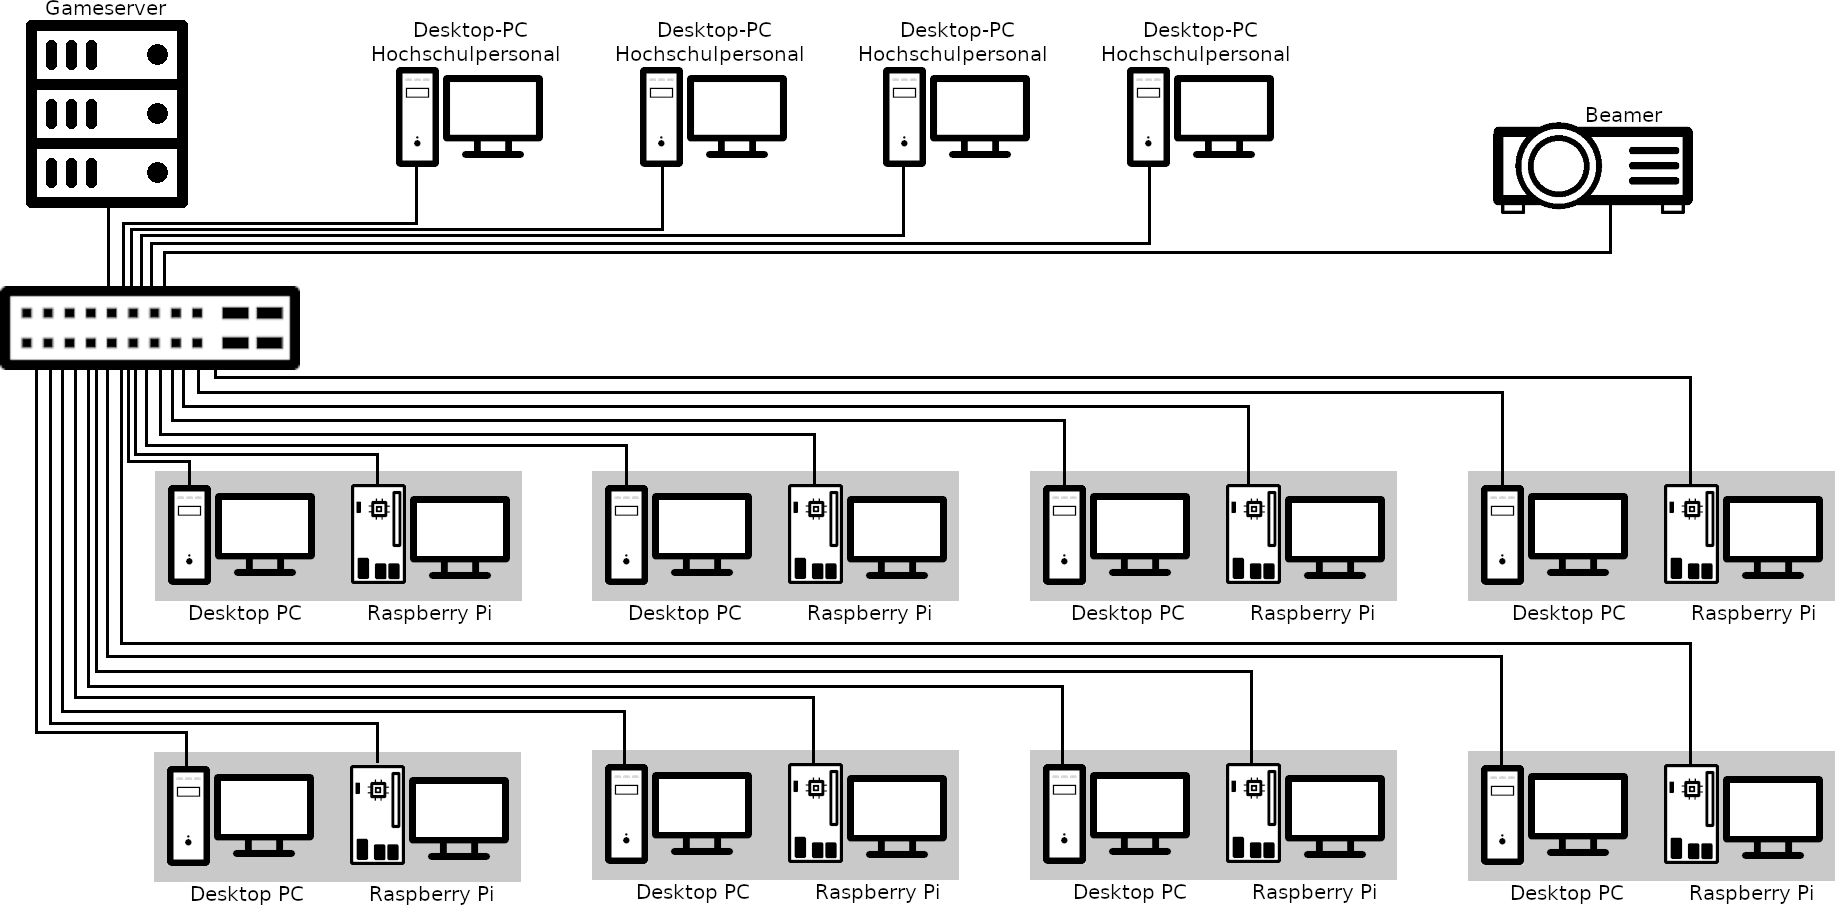
\includegraphics[width=\linewidth, keepaspectratio]{analyse/netzwerk-topologie-bak}
	\captionof{figure}{Übersicht über die Laborausstattung (Netzwerktopologie)}
	\label{fig:network-topology}
\end{center}

Wie in der \autoref{fig:network-topology} dargestellt, ist das Labor mit acht Gruppenarbeitsplätzen für Studierende sowie Arbeitsplätzen für die Mitarbeitenden ausgestattet. Ein Arbeitsplatz kann zu einem neunten Gruppenarbeitsplatz umfunktioniert werden.

An einem Gruppenarbeitsplatz (in der Abbildung \ref{fig:network-topology} grau hinterlegt) können 2 Studierende gleichzeitig arbeiten, da diese mit einem leistungsfähigen Desktop-PC und einem Raspberry Pi\footnote{Einplatinencomputer mit der Größe einer Kreditkarte} sowie den dazugehörigen Peripheriegeräten (Maus, Tastatur \& Monitor) ausgestattet sind.

Als Betriebssystem wird auf den Desktop-PCs Ubuntu\footnote{Ubuntu ist eine freie Linux Distribution auf Basis von Debian} und auf den Raspberry Pis Raspbian\footnote{Abwandlung von Debian für den Raspberry Pi} verwendet.

Auf den Desktop-PCs ist die Software VirtualBox der Firma Oracle installiert. Diese ermöglicht das Virtualisieren eines weiteren Rechners. Diese virtuelle Maschine wird Gast genannt und beheimatet die Dienste und Anwendungen, welche während des Versuchs benötigt werden. Durch die Nutzung der Virtualisierung muss die Software nicht auf dem Wirtsystem installiert werden. So ist dieses auch für andere Versuche im Rahmen der Lehrveranstaltung nutzbar, ohne dass auf Inkompatibilitäten von Softwares der verschiedenen Versuche geachtet werden muss. Auch bietet VirtualBox die Möglichkeit sogenannte Snapshots anzulegen. Ein Snapshot ist eine Momentaufnahme eines aktuellen Systemzustandes. Diese stellt eine Komplettsicherung des Systems dar und es ist möglich, die Systeme auf den gleichen Stand zu bringen. \cite{oraclecorporationOracleVMVirtualBox2020} Dies wird benötigt, um eine Vergleichbarkeit zwischen den Studierenden zu gewährleisten.

Die teilnehmenden Studentengruppen werden in den Softwarekomponenten und in der Auswertung durch die IP-Adresse ihres Gast-Systems identifiziert.

Neben diesen Rechner steht ein Linux Server zur Verfügung, auf welchem das Auswertungs- und Überwachungssystem betrieben wird.

Alle Rechner, auch die Gastsysteme der Studentengruppen, sind untereinander über ein Netzwerkswitch via Ethernet verbunden.

Außerdem steht ein Beamer zur Verfügung, auf dem die aktuelle Spielübersicht dargestellt werden kann.
	\section{Versuch: Catch me, if you can}
\label{sec:Versuch}

Der zweite der drei Versuche \textquote{Catch me, if you can} wird im Rahmen eines Wettbewerbs zwischen den teilnehmenden Studierendenteams ausgetragen. Der Wettbewerb ist an ein Capture the Flag (CTF) angelehnt. Bei einem klassischen CTF erhält der Spielende durch das Lösen von Aufgaben einen bestimmten Text. Dieser wird Flag genannt. Die Aufgaben können das Lösen einer Art Schnitzeljagd, eine einfache Programmierung, aber auch das Hacken mehrerer entfernter Rechner umfassen. Anders als beim klassischen CTF werden bei \textquote{Catch me, if you can} die Flags auf allen teilnehmenden Systemen verteilt. \cite{tanWhatCTFHow2020} Die Studierenden können diese durch das Analysieren ihres eigenen Gastsystems sowie durch den Angriff auf fremde Gastsysteme erhalten. Besonderheit hierbei sind die Strafpunkte für den Verlust einer Flag an gegnerische Studierendenteams. Wie beim klassischen CTF können die Studierenden Flags und Punkte durch zentrale Aufgaben erhalten.

\newpage

Der Versuch ist in drei Phasen untergliedert.
\begin{enumerate}
	\item Vorbereitung
	\item Wettbewerb
	\item Abschluss
\end{enumerate}

\subsubsection{Vorbereitung}
Die Studierenden erhalten circa 30 Minuten Zeit, um ihr Gastsystem in Betrieb zu nehmen und sich mit diesem vertraut zu machen. Hierbei sollten die Schwachstellen in den vorhandenen Diensten abgesichert und der Zugriff durch andere Studierende verhindert werden. Während dieser Zeit dürfen die Studierenden andere Systeme nicht angreifen. Auch ist es möglich, in dieser Zeit Flags auf dem eigenen System der Studierenden zu suchen. Da der Ablageort der Flags auf allen Systemen gleich ist, kann diese Information im Spielverlauf bei einem eigens initiierten Angriff schneller Flags einbringen.

\subsubsection{Wettbewerb}
Die Wettbewerbsphase selbst dauert circa 140 Minuten. In dieser Zeit sind Angriffe auf fremde Gastsysteme erlaubt und ausdrücklich erwünscht. Eine weitere Absicherung ist ebenfalls möglich. Das System sollte auf fremde Aktivitäten hin überwacht werden. Diese Aktivitäten sollten schnellstmöglich unterbunden werden, da die Angreifer Flags entwenden können und so dem Team Strafpunkte einbringen. Auch kann die Zeit für die Lösung von zur Verfügung stehenden Challenges sowie die Nutzung des Flagshops genutzt werden. Der Flagshop sowie die Challenges werden im nächsten Kapitel aufgegriffen.

\subsubsection{Abschluss}
Nach Ende der Wettbewerbsphase müssen die Studierenden ihre Angriffe einstellen und eine weitere Flagabgabe ist nicht mehr möglich. Die Studierenden erstellen für ihren anzufertigen Versuchsbericht einen Screenshot der Punkteübersicht. Eine Nachbesprechung ist optional und auf maximal 30 Minuten begrenzt.

Während des Wettbewerbs gelten die aufgelisteten Regeln. Es handelt sich hierbei nur um einen Auszug der für die Bachelorarbeit relevanten Regeln.
\begin{itemize}
\item Der Gameserver darf nicht angegriffen werden
\item Es dürfen nur die Gastsysteme angegriffen werden
\item Das Passwort des Logins \textit{gamemaster} darf nicht zurückgesetzt werden
\item Der SSH-Server muss für alle erreichbar sein
\item Flags dürfen nicht modifiziert oder gelöscht werden
\item Sämtliche Dienste müssen für den Gameserver erreichbar bleiben
\item ICMP-Pakete (ping) dürfen nicht blockiert werden.
\end{itemize} \cite[S.9]{quadePraktikumITSecurity2017} \cite[S.10-11]{sosnaKonzeptionUndRealisierung2010}
	\section{Systemkomponenten}\label{sec:Systemkomponenten}

\subsection{Komponenten des Servers}\label{subsec:Komponente_des_Servers}
Im Folgenden werden die verschiedenen Komponenten des Auswertungs- und Überwachungssystems in der derzeitigen Implementierung untersucht. Dabei werden Rückschlüsse auf Anforderungen gezogen sowie Schwachstellen herausgearbeitet.

\subsubsection{Scanner}\label{subsubsec:Scanner}
Der Scanner prüft in regelmäßigen Abständen die auf den Gastsystemen der Studierenden installierten Dienste und speichert das Ergebnis ab. Die Abstände können beim Starten des Spieles eingestellt werden. Die folgenden Dienste werden pro Team geprüft.

\paragraph{ScanUp}\label{para:ScanUp}
Die Aufgabe dieses Scans besteht darin zu prüfen, ob das Gastsystem noch für den Server erreichbar ist. Sollte das Gastsystem nicht erreichbar sein, wird hierfür ein Strafpunkt vergeben. Aus technischer Sicht wird das Linux-Kommando \textit{ping} verwendet. Anhand des Rückgabewertes kann nachvollzogen werden, ob der Server das Gastsystem erreichen konnte.

\paragraph{ScanBubble}\label{para:ScanBubble}
Auf dem Gastsystem läuft ein selbst programmierter Bubble Server, welcher Flags unter Nutzung des Telnet Protokolls bereitstellt. Nachdem eine Flag abgeholt wurde, stellt der Dienst für eine bestimmte Zeit (Timeout) keine weiteren Flags bereit. Der Bubble Server nimmt Anfragen über den Port \textit{12321} für unverschlüsselte Flags und Port \textit{12322} für verschlüsselte Flags entgegen. Die Scan-Operation überprüft, ob eine Telnet-Verbindung zum Port \textit{12321} möglich ist, indem die Operation eine Telnet-Verbindung öffnet und prüft, ob die Verbindung erfolgreich war.
\newpage

\paragraph{ScanWebUp}\label{para:ScanWebUp}
Jedes Gastsystem stellt unter Zuhilfenahme eines Apache-Webservers und php-Dateien Webseiten und Daten bereit, die über einen Webclient abgerufen werden können. Dazu müssen auf Port \textit{80} der HTTP- und auf Port \textit{443} der HTTPS-Dienst laufen und erreichbar sein. Dieses verifiziert die Scan-Operation, indem sie eine Socket-Verbindung zu den Ports \textit{80} und \textit{443} öffnet und das Ergebnis prüft.

\paragraph{ScanSQLInjectUp}\label{para:ScanSQLInjectUp}
Dieser Scan prüft, ob die Login-Seite des Teams, auf der die SQL-Injection-Schwachstelle implementiert ist, erreichbar und benutzbar ist. Die Operation sendet hierzu eine valide Kombination aus Nutzername und Passwort an den Webserver. Das Ergebnis wird dann mit dem erwarteten Resultat verglichen.

\paragraph{ScanSQLInjectSave}\label{para:ScanSQLInjectSave}
Ähnlich wie bei der Operation ScanSQLInjectUp (\ref{para:ScanSQLInjectUp}) wird geprüft, ob Ergebnis und Erwartung übereinstimmen. Besonderheit hierbei ist, dass statt einer validen Kombination aus Nutzernamen und Passwort eine sogenannte SQL-Injection (wird im \autoref{subsec:Komponente_des_Clients} genauer erläutert) im Nutzernamen übergeben wird.  
Sollte die Anfrage alle gespeicherten Nutzerdaten zurückgeben, ohne dass eine Authentifizierung stattfindet, ist die SQL-Injection weiterhin möglich.

\paragraph{ScanXSSSave}\label{para:ScanXSSSave}
Diese Scan-Operation prüft, ob die auf dem Gastsystem implementierte XSS-Schwachstelle behoben wurde. Dazu wird die Webseite mit präpariertem Inhalt aufgerufen. Auf die Vorgehensweise wird im \autoref{subsec:Komponente_des_Clients} eingegangen.
In der Rückgabe wird geprüft, ob dieser ungefiltert auf der Webseite zu finden ist. Sollte dies der Fall sein, ist die XSS-Schwachstelle nicht oder unzureichend von den Studierenden abgesichert worden.

\paragraph{ScanSQLSave}\label{para:ScanSQLSave}
Bei diesem Scan wird kontrolliert, ob der Login mit dem auf allen Systemen voreingestellten Passwort \textit{toor} für den SQL-Account \textit{root} möglich ist. Ist dieser möglich, haben die Studierenden dieses unsichere Passwort nicht geändert. Des Weiteren wird geprüft, ob die Nutzerdaten in der htaccess-Datei, die die phpMyAdmin-Anwendung schützen soll, geändert worden sind.

\paragraph{ScanFTPSave}\label{para:ScanFTPSave}
Auf dem Client System läuft ein FTP-Server, der ohne Login (Nutzername \& Passwort) Daten bereitstellt. Der Scan prüft, ob ein sogenannter anonymer Login möglich ist, indem eine FTP-Verbindung ohne Login aufgebaut wird. Sollte die Verbindung erfolgreich sein, ist der anonyme Login immer noch nicht deaktiviert worden.

\paragraph{ScanTelnetSave}\label{para:ScanTelnetSave}
Ein Telnet-Server horcht auf Verbindungen auf Port \textit{23}. Da dieser Dienst nicht benötigt wird, soll er durch die Studierenden abgeschaltet oder deinstalliert werden. Die Scan-Operation prüft, ob eine Verbindung mithilfe des Telnet-Protokolls auf Port \textit{23} möglich ist. Dazu wird eine Verbindung zu Port \textit{23} aufgebaut und das Resultat geprüft.

\subsubsection{Generierung von Flags}\label{subsubsec:Generierung_von_Flags}

Derzeitig erfolgt die Generierung der Flags sowohl auf den Gastsystemen als auch auf dem Auswertungs- und Überwachungssystem. Dies ist notwendig, da ansonsten eine Überprüfung der Gültigkeit der Flags und Verrechnung der Punkte nicht durchgeführt werden kann. Die Flags werden durch einen Algorithmus generiert. Dieser erzeugt pro Team eine bestimmte Anzahl an Flags. 

Dazu wird die Flag mithilfe der Streuwertfunktion (Hashfunktion) MD5 und der Eingabe, einem sogenannten Seed, berechnet. Eine Hashfunktion bildet aus einer Eingabe variabler Länge eine Ausgabe mit einer festen Länge. Bei identischer Eingabe wird immer der gleiche Ausgabewert berechnet. Darüber hinaus ist es bei einer guten Hashfunktion nicht möglich, von der Ausgabe auf den Eingabewert zu schließen. \cite{menezesHandbookAppliedCryptography1996}

Der in der Anwendung genutzte Seed setzt sich aus der Verkettung von \textit{Salt}, \textit{IP-Adresse}, dem String \textquote{\textit{Aufgabe}} und einem \textit{Zähler} zusammen.

\begin{lstlisting}[, frame=single, caption={Beispiel eines Seed und seines Hashs}, captionpos=b, label={lst:analyse-hash-algo}]
seed = "WS2019192.168.87.11Aufgabe1"
hash = md5(seed)
hash = 7072D70B3D47E8516056A8B777655174
\end{lstlisting}

Ein Salt wird benötigt, um den Flags eine Lebenszeit zu geben. In der derzeitigen Implementierung enthält der Salt das aktuelle Jahr sowie das jeweilige Semester. So sind nur Flags des aktuellen Semesters gültig und werden vom Auswertungs- und Überwachungssystem akzeptiert. Einer Verwendung von Flags aus vorherigen Semestern wird somit effektiv vorgebeugt.

Die IP-Adresse stellt hierbei den Bezug zum jeweiligen Team dar.

Der String \textquote{Aufgabe} wird als Geheimnis verwendet, um das Fälschen von Flags zu erschweren und bestenfalls zu verhindern.

Damit pro Team mehrere eindeutige Flags generiert werden können, wird ein sogenannter Zähler genutzt. Dieser Zähler ist auf 0 initialisiert und wird pro generierter Flag um eins erhöht, bis die benötigte Anzahl an Flags generiert ist. \cite[S.48]{sosnaKonzeptionUndRealisierung2010}

\subsubsection{Webserver}\label{subsubsec:Webserver}

Der Webserver stellt das GUI (Graphical User Interface) für die Studierenden und betreuenden Personen dar. Hier kann der aktuelle Punktestand eingesehen werden. Auch wird in dem GUI dargestellt, welches Team welchen Service abgesichert hat, inklusive der Negativpunkte für nicht abgesicherte Dienste, und wie viele Strafpunkte das jeweilige Team erhalten hat.

Neben diesen Darstellungen befinden sich auf dem Server ein sogenannter Flagshop und diverse Challenges, mit denen Studierende weitere Flags erhalten können.

Die betreuenden Personen haben die Möglichkeit, über das Web-GUI ein neues Spiel anzulegen und das Spiel zu starten oder zu stoppen. Auch kann von dem Spiel ein Backup erstellt werden. Neben diesen Funktionen zur Spielsteuerung können an die Teams Strafen für unfaires oder regelverletzendes Verhalten verteilt werden. Diese nehmen direkten Einfluss auf die Punkte des jeweiligen Teams. Außerdem besteht die Möglichkeit, weitere Benutzer für das Administrationsinterface zu registrieren.

\paragraph{Flagshop} \label{para:Flagshop}
Der Flagshop ermöglicht es den Studierenden, weitere Flags mit ihren Punkten zu kaufen. Der Kauf von Flags lohnt sich, da die verkauften Flags mehr Punkte bringen als sie kosten. Um einen Einkauf im Flagshop durchzuführen, müssen die Teams vorher einen Account erstellen. Die Registrierung erfragt neben dem benötigten Benutzernamen und Passwort auch für den Flagshop irrelevante Daten ab. Diese ähneln persönlichen Informationen, die bei den meisten Onlineshops angegeben werden müssen. Das Format, hier die Repräsentation als Zahl oder String sowie die Länge, und die Erforderlichkeit der Daten werden nur im HTML-Formular festgelegt. Durch eine Manipulierung des Formulars kann dieses mit nicht konformen oder nicht vorhandenen Daten abgesendet werden. Für jede der nicht vorhandenen oder nicht konformen Informationen erhält der Studierende eine Flag. Daneben wird die \linebreak Güte des angegebenen Passwortes anhand von Länge und Anzahl an Sonderzeichen, Groß- und Kleinbuchstaben sowie Ziffern bewertet und mit Flags belohnt.

Nach der Registrierung können die Studierenden sich für ihre Punkte Flags kaufen. Dazu stehen zwei Pakete mit 8 bzw. 6 Flags für den Preis von jeweils 4 Punkten pro Paket zur Verfügung. Dieser Preis kann auf zwei Arten reduziert werden. 
Einmal müssen sich die beiden Pakete gleichzeitig im Warenkorb befinden und deren Identifikationsnummern (ID) müssen auf nicht vorhandene Nummern gesetzt werden. Die Manipulation resultiert in einem reduzierten Preis von 4 Punkten für beide Pakete. Dies ist extra im Flagshop einprogrammiert und soll die Studierenden auf Manipulation von IDs aufmerksam machen.
Durch die zweite Art ist es möglich, die Pakete kostenlos zu erhalten. Dazu muss im Warenkorb das sogenannte \textit{Hidden-Input-Feld}, in dem der aktuelle Preis des Warenkorbs gespeichert wird, auf 0 gesetzt werden. Dann berechnet der Flagshop für den Kauf einen Preis von 0 Punkten. \cite[S. 63]{abtsUeberarbeitungUndErweiterung2016}

Ein \textit{Hidden-Input-Feld} wird in der Repräsentation eines HTML-Dokumentes nicht angezeigt, kann jedoch durch die Entwicklertools eines Browser betrachtet und verändert werden. \cite{w3schoolsHTMLHiddenInput}

Auf diese Weise ist es auch möglich, einen negativen Preis festzulegen und dem eigenen Team Punkte zuzuschreiben, da die derzeitige Implementierung nicht prüft, ob der von dem Nutzenden eingegebene Preis kleiner als 0 ist, sondern ob dieser gleich 0 ist. Bei korrekter Implementierung würde ein Preis kleiner 0 geprüft und korrigiert.

\paragraph{Challenges} \label{para:Challenges}
Derzeitig sind fünf Challenges implementiert, die vom System in zufälliger Reihenfolge an interessierte Teams verteilt werden. Eine abgeschlossene oder abgebrochene Challenge, durch das Neuladen der Webseite oder durch das Betätigen der Zurück-Taste, kann nicht wiederholt werden. Eine Challenge kostet 10 Punkte. Nach erfolgreichem Abschluss einer Challenge gibt es 10 Punkte plus eine gewisse Anzahl an Punkten für das Absolvieren der Aufgabe. Die folgenden Challenges sind implementiert: \cite[S.19]{abtsUeberarbeitungUndErweiterung2016}

\subparagraph{Aufgabe 1: robots.txt}\label{subpara:Aufgabe_1_robots.txt}
Die Studierenden sollen in dieser Challenge lernen, dass die \textit{robots.txt} Datei keinen Zugriffsschutz darstellt. Diese bittet nur Suchmaschinen, die angegebenen Verzeichnisse und Dateien nicht zu indexieren. Aus der \textit{robots.txt} Datei können Informationen zu versteckten Dateien und Verzeichnissen erhalten werden. Die Studierenden sollen über die \textit{robots.txt} Datei einen vorhandenen Ordner finden. In diesem befindet sich die Lösung zur Challenge. \cite[S.19-20]{abtsUeberarbeitungUndErweiterung2016}

\subparagraph{Aufgabe 2: JavaScript-Login-Bypass}\label{subpara:Aufgabe_2_JavaScript-Login-Bypass}
Bei dieser Challenge ist das benötigte Passwort zur Lösung der Challenge als Klartext im Quelltext versteckt. Das Verstecken wird derzeitig mit einer Meldung wie \textquote[\cite{abtsUeberarbeitungUndErweiterung2016}]{Seitenquelltext deaktiviert} und vielen Leerzeilen realisiert. Im Inspector von Firefox Version 78.0.1 und Chromium Version 83.0.4103.116 ist dies nicht möglich, da die Leerzeilen entfernt werden und das Passwort daher oben im Quelltext zu sehen ist. \cite[S.20]{abtsUeberarbeitungUndErweiterung2016}

\subparagraph{Aufgabe 3: Form-Modification}\label{subpara:Aufgabe_3_Form-Modification}
In dieser Challenge sollen die Studierenden verstehen, dass auch die Werte von Drop-Down-Menüs, Checkboxen und Radio-Buttons durch Manipulation auf nicht vorgegebene Werte geändert werden können. Deshalb müssen Nutzereingaben stets auch serverseitig überprüft werden, da hier die Regeln der Überprüfung nicht durch den Nutzenden verändert werden können.

Die Aufgabe besteht darin, einen bestimmten Login-Namen aus einem Drop-Down-Menü auszuwählen. Da der geforderte Name nicht in dieser Liste ist, müssen die Studierenden das HTML-Formular so manipulieren, dass er auswählbar ist. \cite[S.20]{abtsUeberarbeitungUndErweiterung2016}

\subparagraph{Aufgabe 4: JavaScript-Substrings}\label{subpara:Aufgabe_4_JavaScript-Substrings}
Das Passwort, das die Studierenden eingeben müssen, wird clientseitig mithilfe einer JavaScript Funktion geprüft. Damit das Passwort nicht im Klartext im Quelltext steht, wird dieses verschleiert. So werden drei Strings Zeichen für Zeichen verglichen. Sollte ein Zeichen in mindestens zwei der drei Strings übereinstimmen, dann gehört dieses Zeichen zum Passwort. Im Anschluss wird geprüft, ob das generierte Passwort gleich dem ist, das die Studierenden als Passwort genutzt haben. \cite[S.20]{abtsUeberarbeitungUndErweiterung2016}

\subparagraph{Aufgabe 5: URL-Hex-Injection}\label{subpara:Aufgabe_5_URL-Hex-Injection}
Die Studierenden sollen an geheime Informationen in einem Ordner gelangen, der nach einem Wert aus dem Hexadezimalsystem benannt ist. Anders als im Dezimalsystem ist die Basis 16 statt 10. Die Aufgabe soll zeigen, dass Ordner, die nach einem Hexadezimalwert benannten sind, auf diese Art und Weise nicht vor Zugriffen geschützt werden können, da das Präfix Zeichen \textit{\%} für Hexadezimalzahlen selbst durch einen Hexadezimalwert (\%25) dargestellt werden kann. \cite[S.20]{abtsUeberarbeitungUndErweiterung2016}

\subsubsection{Abgabe von Flags}\label{subsubsec:Abgabe_von_Flags}
Um Flags abgeben zu können, müssen die Studierenden sich mit ihren Zugangsdaten, die sie durch das Lösen des Hackits erhalten haben, in der Web-GUI anmelden. Dort ist es möglich, in einem Input-Feld eine Flag synchron abzugeben. Das bedeutet, dass nach jeder Abgabe die Webseite neu geladen wird. Eine Abgabe mehrere Flags ist gleichzeitig nicht möglich.

\subsection{Komponenten des Clients}\label{subsec:Komponente_des_Clients}
Da sich die Bachelorarbeit mit der Modernisierung des Auswertungs- und Überwachungssystems beschäftigt, sind nur die für die Bachelorarbeit wichtigen Komponenten des Clients beschrieben.

\subsubsection{Webserver des Clients}\label{subsubsec:Webserver_des_Clients}
Auf den Clients wird ein Webserver mit einigen extra implementierten Schwachstellen betrieben. Diese sollen während des Versuches durch die Studierenden behoben werden.

Der Webserver stellt eine Art Kundenbewertungsformular mit implementierter XSS Schwachstelle bereit. In der verwendeten Implementierung wird die Eingabe des Nutzers in das HTML-Dokument geschrieben. Durch die Schwachstelle wird eine Nutzereingabe ungefiltert in das HTML-Formular übernommen und ein potenziell schädlicher Code wird vom Browser verarbeitet. Dieser Code kann dann beispielsweise vertrauliche Informationen wie Cookies, Session-Tokens oder persönliche Daten auslesen und den Angreifern übermitteln. \cite{ruettenSicherheitWebanwendungen2007}

Eine weitere Schwachstelle stellt der sogenannte \textquote{Login zum Membersbereich} mit der implementierten SQL-Injection Schwachstelle dar. 
Bei einer SQL-Injection versucht ein Angreifer den verwendeten SQL-Befehl so zu erweitern, dass dieser neben der eigentlichen Abfrage an die Datenbank auch einen vom Angreifer vorbereiteten SQL-Befehl ausführt. Die Erweiterung des SQL-Befehls erfolgt, indem die Eingabe, die in den SQL-Befehl aufgenommen wird, das Zeichen für das Ende des SQL-Befehls inklusive des vom Angreifer intendierten SQL-Befehls enthält. Über diesen Angriff können dann unerlaubterweise Daten ausgelesen werden, aber auch eine Löschung der Daten ist denkbar. \cite{bachfeldGiftspritze2004}

In der verwendeten Implementierung werden der Benutzername und das Passwort ungefiltert in den SQL-Befehl übernommen. Diese Schwachstelle lässt sich erst beheben, wenn die Gruppe die SQL-Injection bei sich selbst erfolgreich durchgeführt hat. \cite[S.27-29]{abtsUeberarbeitungUndErweiterung2016}

Neben diesen Schwachstellen gibt es eine Registrierung für den Flagshop. Diese erfordert einige Eingaben wie Name, Alter, Postleitzahl und vieles mehr. Die Eingaben sind im HTML-Formular als Pflicht markiert und haben eine Vorgabe in der Form. Ein Absenden ist ohne Angabe dieser Daten nicht möglich. Die Studierenden erhalten jedoch für jede nicht getätigte und für jede nicht der Form entsprechenden Angabe Flags nach der Registrierung. \cite[S.26]{abtsUeberarbeitungUndErweiterung2016} Dies ist möglich, da das HTML-Formular durch die Studierenden geändert werden kann und der Server nur die Angaben bezüglich Passwort und Nutzername prüft. Diese beiden Angaben werden genutzt, um sich am Flagshop des Servers anzumelden und Flags zu erwerben. \textit{(Siehe: \autoref{para:Flagshop} Flagshop)}

Außerdem stellt der Webserver eine Bildergalerie zur Verfügung. In dieser befinden sich zum Spielstart zwei normal erscheinende Bilder. Entgegen dem Anschein sind in diesen Flags verschleiert. Die Steganografie wird durch die Kombination eines Bildes und eines ZIP-Archivs erreicht. \cite[S.27]{abtsUeberarbeitungUndErweiterung2016}
	\section{Schnittpunkte zwischen Server und Clients}
\label{sec:Schnittpunkte_zwischen_Server_und_Clients}

Der Server und die Clients laufen auf getrennten Systemen. Da die Studierende Schwachstellen auf ihren Clients beheben sollen, muss das Auswertungs- und Überwachungssystem auf diese Systeme zugreifen. Dadurch lassen sich die folgenden Schnittpunkte begründen.

Die Scanner prüfen vom Auswertungs- und Überwachungssystem aus, ob 
\begin{itemize}
	\item das System online ist,
	\item der Webserver erreichbar ist,
	\item der Bubble-Server erreichbar ist,
	\item der Login zum Membersbereich erreichbar und abgesichert ist,
	\item die Kundenbewertung erreichbar und abgesichert ist,
	\item ob das SQL Passwort geändert worden ist,
	\item ob der FTP Server gegen unautorisierten Zugriff abgesichert ist und
	\item ob der Telnet Dienst auf Port 23 abgeschaltet ist. 
\end{itemize}

Des Weiteren verbinden sich die Clients beim Starten mit dem Auswertungs- und Überwachungssystem um Flags für die Flagshop-Registrierung und -Anmeldung zur Verfügung zu stellen.
	\section{Abgeleitete Anforderungen}
\label{sec:Abgeleitete_Anforderungen}

Das Auswertungs- und Überwachungssystem muss anhand der vorhergehenden Analyse folgenden Anforderungen genügen:
\begin{itemize}
	\item Überwachung von mindestens neun Studierendensystemen
	\item Ermittlung und Sicherung der Zustände von Diensten, welche auf den Studierendensystemen angeboten werden müssen
	\item Entgegennahme und Prüfung von Flags, inkl. der Verrechnung von (Straf-)Punkten
	\item Ermittlung und Visualisierung der Teilergebnisse sowie des Gesamtergebnisses
	\item Informationsvermittlung aller Dienst- und Punkteänderungen durch unter anderem \\ Dienststatusänderung, Flagabgabe und Strafen (fortlaufende Publikation für Studierende und betreuende Personen)
	\item Dokumentation aller Events durch Protokollierung der einzelnen Aktionen des Systems
	\item Bereitstellung von Challenges, damit Studierende sich weitere Punkte erarbeiten können
	\item Bereitstellung eines (Flag-) Shops, bei dem mehrere Sicherheitslücken ausgenutzt werden können, um Flags zu erhalten
	\item Einstellungen des Spiels sollen durch betreuende Personen geändert werden können
	\item Verwaltung von Benutzern (administrierende, betreuende und spielende Personen)
	\item Zugangskontrolle für teilnehmende Studierende durch Prüfung der Hackits
	\item Sicherung alter Spielstände.
\end{itemize}
	
	\chapter{Entwurf}
	\label{chap:Entwurf}
	Dieses Kapitel beinhaltet die Architektur des Systems sowie den Entwurf der einzelnen Komponenten.

Es wird die Struktur und Zusammensetzung des Systems sowie der einzelnen Komponenten skizziert. Auch werden die Anforderungen und Erwartungen an die verschiedenen Systemkomponenten dargestellt.

Bei einigen Komponenten werden auch Alternativen aufgezeigt, welche auf Grundlage der genannten Entscheidungen im Entwurf nicht verwendet worden sind.
	\section{Entwurfsziele} \label{sec:Entwurfsziele}

Bei dem Entwurf des neuen Systems sind neben den in der Analyse beschrieben Anforderungen auch folgende Ziele beachtet worden.

\paragraph{Beibehaltung der Features}
Die bereits implementierten Features Flagshop und Challenges sollen auch im neuen System verfügbar sein. Zusätzlich sollen die Studierenden aktiv angeregt werden diese auch zu nutzen.

\paragraph{Lose Kopplung}
Zwischen dem Scanner und dem Webserver soll eine lose Kopplung herrschen, damit die Entwicklung der beiden Komponenten unabhängig voneinander fortgesetzt werden kann.

\paragraph{Datenhaltung in Datenbank}
Die Nutzung einer Datenbank sollte aufgrund zweier Überlegungen angestrebt werden. Erstens sind alle Daten an einem Ort gebündelt. Zweitens kann die Berechnung von Punkten an die Datenbank abgeben werden. Datenbanken sind unter anderem für solche Aufgaben geeignet.

\paragraph{Modernisierung der GUI}
Das Graphical User Interface soll modernisiert werden, sodass es heutigen Standards entspricht. Auch soll hierdurch die Verständlichkeit verbessert und die Challenges sowie der Flagshop besser platziert werden.

\paragraph{Einheitliche Programmiersprache}
Eine einheitliche Programmiersprache sollte, sofern dieses möglich ist, genutzt werden. Dieses erleichtert das Betreiben der Komponenten, da nicht zwei verschiedene Programmiersprachen und/oder Umgebungen installiert werden müssen. Auch erleichtert es die Programmierung, wenn nur eine Person parallel an den Komponenten arbeitet. Die Gefahr von falschen Syntaxen und verschiedener Konventionen kann dadurch reduziert werden. Sollte die Anwendung durch mehrere Menschen entwickelt und gewartet werden sowie auf verschiedenen Systemen betrieben werden, ist dieses Ziel nichtig.

\paragraph{Module sparsam nutzen}
Bei der Implementierung der Software sollte so weit dieses notwendig und sinnvoll ist auf bereits vorhandene Module und Frameworks zurückgegriffen werden. Durch die Minimierung von Abhängigkeiten ist die Wartung von Verwendung der Software durch Dritte leichter möglich. Auch wird die Gefahr von Fehler auslösenden Updates minimiert. Bei der Nutzung von Modulen und Frameworks sollte auf deren Verbreitung und Wartung geachtet werden, damit nicht inaktive Module/Frameworks mit eventuellen Schwächen genutzt werden.

\paragraph{Containerisierung}
Die Anwendung soll mit möglichst kleinem Wartungsaufwand überall benutzbar sein. Um dieses zu gewährleisten, sollte eine Containerisierung genutzt werden. Bei der Nutzung ist darauf zu achten, ob und mit welchen Einschränkungen diese nutzbar ist.

\paragraph{Ressourcen schonend}
Um die Ressourcen des Servers zu schonen, sollten die nicht benötigten Komponenten abgeschaltet werden. Hierbei ist der Scanner hervorzuheben, welcher nur während des Praktikums laufen muss. 
	\section{Containerisierung} \label{sec:Containerisierung}
Bei der Containerisierung wird jeder Container als eine eigene logische Maschine betrachtet. Es können mehrere Container gleichzeitig auf einer physischen Maschine betrieben werden. 
Die verschiedenen Container laufen unabhängig voneinander und wissen nicht über die Existenz weitere Container Bescheid. Sollte eine Kommunikation zwischen zwei Container benötigt werden, erfolgt diese über die Netzwerkschnittstelle ähnlich der Kommunikation zwischen Anwendungen, die auf verschiedener physischer Geräte. \cite{boersmaContainerizationDefinitionBest2019} Damit die Container kommunizieren können, muss vorher ein Netzwerk konfiguriert werden, in dem sich die Container gemeinsam befinden.

Im Gegensatz zur Virtualisierung teilen sich die Container das zugrunde liegende Betriebssystem nicht. Dieses reduziert den Verbrauch von Ressourcen wie CPU und Arbeitsspeicher, da diese nur für die Anwendung und nicht das Betriebssystem benötigt werden.

Containerisierung wird verwendet, um Anwendungen getrennt betreiben zu können. So können verschiedene Versionen einer Software gleichzeitig auf der gleichen physischen Maschine betrieben werden, ohne dass es zu Interferenzen kommt oder das veränderte Konfigurationen notwendig sind. Des Weiteren läuft ein Container auf die gleiche Art und Weise unabhängig von der darunter liegenden Hardwarearchitektur. So läuft ein Container auf dem Rechner des Entwickelnden genauso wie ein Container in einem Rechenzentrum. Durch diese Eigenschaft sind die Anwendungen in Containeren portabel. \cite{boersmaContainerizationDefinitionBest2019}

Durch die Isolierungen können Anwendungen keinen negativen Einfluss auf weitere Container nehmen.

Docker wurde erstmalig im Jahr 2013 als Open-Source-Software veröffentlicht und zählt derzeitig zu den am weit verbreitetste Anwendung für Containierisierung. Es ist der de facto Standard für Containierisierung. 
\cite{boersmaContainerizationDefinitionBest2019}

Heutzutage nutzen immer mehr Unternehmen Orchestierungstechnologien wie Kubernetes oder OpenStack um Container zentral über mehrere physische Maschinen zu verwalten und zu skalieren.
\cite{gaviganHistoryAngular2018}

Eine Kubernetes-Installation ist im EZS-Labor bisher noch nicht vorhanden. Auch ist eine Installation für diese Bachelorarbeit aufgrund der Kosten-Nutzen-Differenz nicht empfehlenswert.

Anstatt einer Orchestierungssoftware wird \textit{Docker Compose} genutzt werden.
Mithilfe dieses Tools können mehrere Container zu einem Service zusammengefasst und verwaltet werden. \textit{Docker Compose} wird verwendet um die beiden serverseitigen Anwendungen sowie die beiden Datenbanken zu einem Service zusammenzufassen. Auch sorgt es dafür, dass die Container in einem eigenen virtuellen Netzwerk laufen und nur untereinander kommunizieren können. \cite{dockerinc.OverviewDockerCompose2020} 
	\section{Übersicht} \label{sec:Übersicht}
\begin{center}
	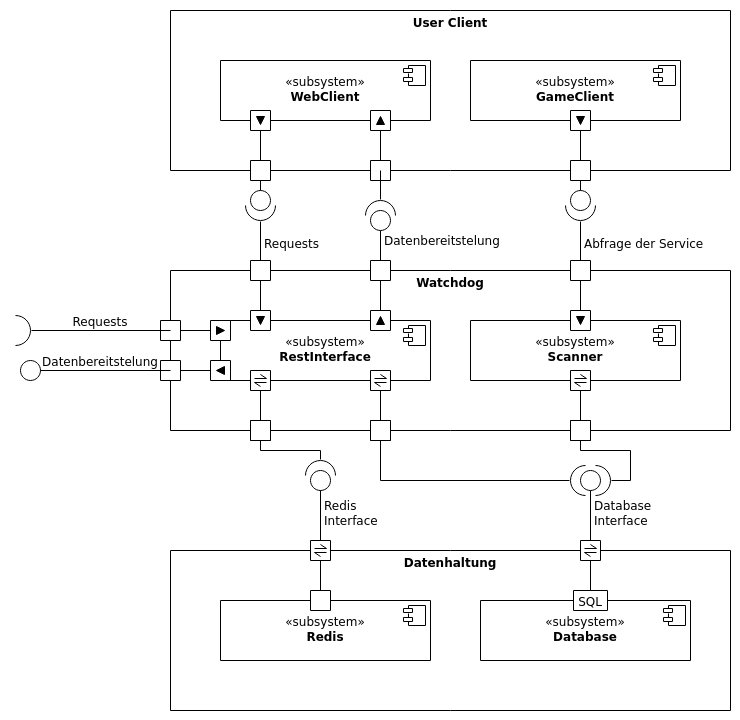
\includegraphics[width=\linewidth, keepaspectratio]{entwurf/uebersicht_component}
	\captionof{figure}{Übersicht über die Anwendung (Komponentendiagramm)}
	\label{fig:system-overview}
\end{center}

Die Gesamtheit des Systems (inklusive der User Clients), wie in \autoref{fig:system-overview} zu sehen, lässt sich in drei Ebenen einteilen.

\paragraph{User Client}
Die erste Ebene \textit{User Client} beinhaltet die auf einem User Client laufenden und für den Versuch relevanten Komponenten.

Bei der Komponente Webclient handelt es sich um einen geläufigen Webbrowser (häufig wird Firefox genutzt), der Informationen vom \textit{CTF Core System} abruft und Daten an dieses übermittelt.
Zu den Informationen gehören beispielsweise die Spielinformationen, der Spielstand aber auch teilnehmende Gruppen und Einstellungen. Der Webclient übermittelt Daten wie gefundene Flags, Lösungen von Aufgaben und Änderungen an Einstellungen.

Die Komponente \textit{GameClient} beinhaltet alle auf dem System für den Versuch installierte Anwendungen. Dazu zählen nicht nur die Dienste mit den Schwachstellen. Auch die clientseitige Spielverwaltungs-Software wird unter dieser Komponente zusammengefasst. Die Spielverwaltungs-Software sorgt für die richtige Konfiguration des User Clients und verteilt bzw. versteckt die Flags.

\paragraph{CTF Core System}
Die Ebene des \textit{CTF Core System} besteht aus den Komponenten \textit{Big Brother} und \textit{Game Information System}. 

Die Komponente \textit{Big Brother} implementiert einen Scanner, der für die Überwachung des \textit{GameClients} mit seinen Schwachstellen zuständig ist. Die Ergebnisse werden in der Komponente \textit{Database} für die Bewertung und Dokumentation festgehalten.

Die zweite Komponente \textit{Game Information System} stellt eine Schnittstelle zwischen der Datenbank und den Nutzern dar. Mithilfe dieser können Informationen unter Berücksichtigung von Berechtigungen auf einem einheitlichen Weg aus der Datenbank ausgelesen, verändert und hinzugefügt werden. 

\paragraph{Datenhaltung}
Die Ebene \textit{Datenhaltung} beinhaltet die Komponenten \textit{Redis} und \textit{Database}. 

Die Komponente \textit{Redis} ist nach der gleichnamigen Software Redis benannt. Bei Redis handelt es sich auch um eine Datenbank und könnte daher mit in die Komponente \textit{Database} aufgenommen werden; die Trennung erfolgt aber auf der Grundlage der Verwendung innerhalb der Software-Architektur. Die Redis-Datenbank wird als Cache verwendet und persistiert die Daten nicht auf der Festplatte, sondern im Hauptspeicher.

Anders als bei Redis werden in der Komponente \textit{Database} die Daten auf eine Festplatte geschrieben, um diese persistent nutzen zu können.
	\section{Scanner} \label{sec:Scanner}
Im Rahmen des Versuches sollen die Studierenden ihre Systeme auf Schwachstellen untersuchen. Diese ausfindig gemachten Schwachstellen sollen im Anschluss beseitigt werden. Eine Überwachung wird benötigt, um zu prüfen, ob die Studierenden diese Schwachstellen behoben haben. Das Abschalten, beziehungsweise die Verhinderung der Verwendung eines Dienstes, stellt in den meisten Fällen keine Behebung der Schwachstelle dar und wird deshalb ebenfalls geprüft. Um diese Überprüfung zu ermöglichen, wird ein Scanner benötigt, der die Dienste auf alle teilnehmenden \textit{GameClients} abfragt und auswertet. Die bei der Überprüfung gesammelten Daten werden benötigt, um die Servicepunkte der Gruppen zu berechnen.

\subsection{Verteilte Scanner}
Eine Idee für die Lastverteilung des Scanners ist ein verteilter Scanner. Hierbei wird ein Worker Scanner auf jedem GameClient implementiert, welcher das eigene System überwacht. Ein Master Scanner sammelt die von den Worker Scannern erstellten Ergebnisse ein und speichert diese in einer Datenbank ab. 

Der Vorteil des verteilten Scanners ist die Skalierbarkeit, da der Scanner auf dem Server nur von weiteren Scannern die Ergebnisse abholen, jedoch keine Überwachung durchführen muss.

Der verteilte Scanner bringt jedoch auch einige Nachteile mit sich. So muss sichergestellt werden, dass der Scanner auf dem User Client nicht manipuliert worden ist und die Ergebnisse valide sind. Eine solche Überprüfung könnte mithilfe eines \textquote{Fingerabdrucks} geschehen. Jedoch muss dann auch geprüft werden, ob das Programm zur Erstellung des Fingerabdrucks manipuliert worden ist.   Des Weiteren muss gewährleistet werden, dass der auf dem Client laufende Scanner dieselben Antworten und Ergebnisse erhält, wie ein fremder Nutzer. Dies ist notwendig, da die überwachten Services weiterhin von anderen Mitspielenden verwendet werden sollen.

Auf Grundlage der Nachteile, des Aufwandes der Implementierung und der ausreichenden Leistung des zentralen Scanners für den aktuellen Anwendungsfall wird ein verteilter Scanner nicht in Betracht gezogen. Die Idee des zentralen Scanners wird weiterverfolgt.

\subsection{Zentraler Scanner}
Die Herangehensweise des zentralen Scanners vermeidet die vorher beschriebenen Nachteile, da dem Ergebnis des Scanners vertraut werden kann und der Scanner zwangsläufig eine externe Sicht auf das System einnimmt. Dem Ergebnis kann vertraut werden, da es auf einem System ohne Einfluss der Mitspielenden berechnet wird.

\begin{center}
	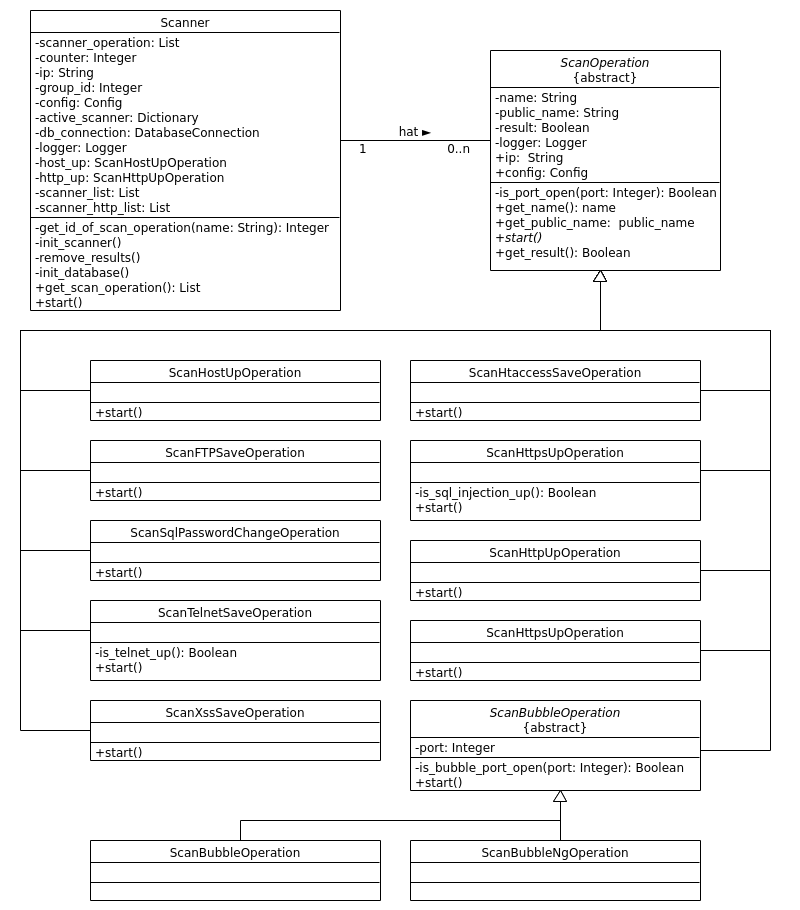
\includegraphics[width=\linewidth]{entwurf/scanner/class_scanner}
	\captionof{figure}{Klassen der Big Brother Komponente (Klassendiagramm)}
	\label{fig:scanner-class}
\end{center}

Wie in Bild \ref{fig:scanner-class} erkennbar besteht die Komponente Big Brother aus der Klasse Scanner, der abstrakten Klasse ScanOperation sowie den abgeleiteten Scan-Operationen.

Die Klasse \textquote{ScanOperation} definiert die abstrakte Funktion \textit{start()}. Diese wird von den abgeleiteten Klassen implementiert und ermöglicht das Starten der einzelnen Scan-Operationen. Ebenfalls speichern alle Scan-Operationen ihr Ergebnis in der privaten Variablen \textit{result}. Mithilfe der von der abstrakten Klasse implementierten Funktion \textit{get\_results()} kann der Scanner das Ergebnis der Scan-Operation auslesen. Jedes Objekt der Klasse Scanner startet 0 bis n Scan-Operationen abhängig von der Konfiguration beziehungsweise den aktiven Diensten. Des Weiteren stellt die abstrakte Klasse die Funktion \textit{is\_port\_open} bereit, welche von den Scan-Operationen genutzt werden kann, um den Status eines Ports auf dem fremden System zu prüfen. Ein Objekt der Klasse Scanner kann pro Typ maximal eine Scan-Operation starten und beinhaltet beziehungsweise verwaltet alle Scan-Operationen für ein Game Client. 

Um mehrere Game Clients zu überwachen, werden mehrere Objekte der Klasse Scanner benötigt.

\begin{center}
	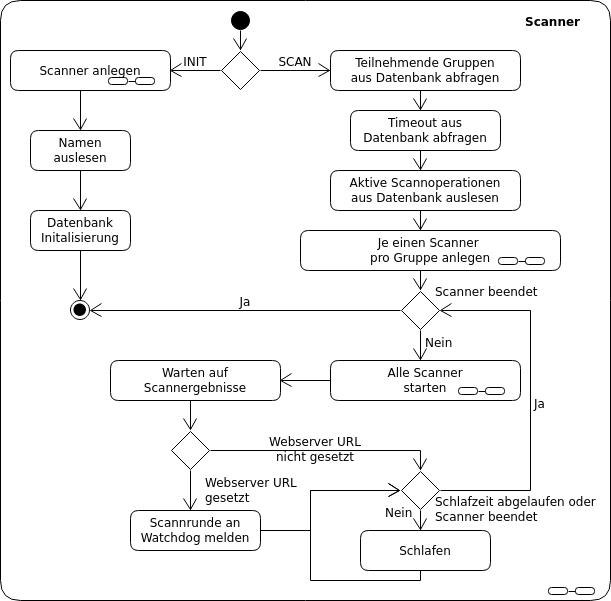
\includegraphics[width=\linewidth]{entwurf/scanner/state_scanner}
	\captionof{figure}{Ansicht des Scanners (Zustandsdiagramm)}
	\label{fig:scanner-state}
\end{center}

Bei Starten des Scanners wird die zu bearbeitende Aufgabe spezifiziert.

Bekommt der Scanner die Aufgabe \textquote{INIT}, soll dieser die Service Datenbank mit den implementierten Scan-Operationen füllen, sodass Administratoren diese an- oder ausschalten können. Um die Service Datenbank zu füllen, wird zunächst ein Dummy der Klasse Scanner angelegt. Aus diesem Dummy Objekt werden von allen Scan-Operationen der Anzeigename und der interne Name ausgelesen. Nach dem Auslesen alle Operationen werden die erhaltenen Daten gebündelt in die Service Datenbank geschrieben. Danach beendet der Scanner die Verbindung zur Datenbank und endet erfolgreich mit dem Statuscode 0.

Falls die Aufgabe des Scanners \textquote{SCAN} ist, wird der Scan der Game Clients gestartet. Hierzu werden die teilnehmenden Gruppen und das Intervall der Scannerdurchgänge aus der Datenbank ausgelesen. Neben diesem werden die aktiven Scanner aus der Datenbank abgefragt. Sind alle Informationen vorhanden, wird für jede Gruppe ein Scanner Objekt der Klasse Scanner erstellt. Bei der Erstellung werden die aktiven Scan-Operationen sowie die zu überwachende Gruppe übergeben. Das Scanner Objekt legt dann für die benötigten Scan-Operationen die jeweiligen Objekte an.

\begin{center}
	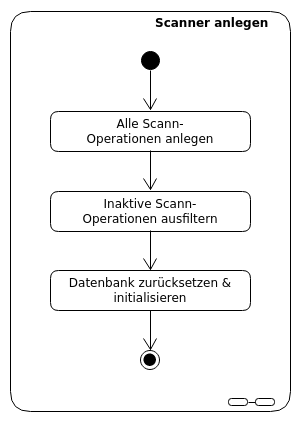
\includegraphics{entwurf/scanner/state_scanner_create}
	\captionof{figure}{Erstellung eines Scanners (Zustandsdiagramm)}
	\label{fig:scanner-create-state}
\end{center}

Nach dem Anlegen aller Scanner wird die Funktion \textit{start()} nebenläufig gestartet. Im Anschluss wird auf das Beenden der gestarteten Funktionen gewartet. Sollten alle abgeschlossen sein, wird geprüft, ob das Durchführen einer Scan-Runde an den Webserver gemeldet werden soll. Ist dies der Fall, wird der Server darüber in Kenntnis gesetzt, dass neue Daten in der Datenbank vorhanden sind. Danach schläft der Scanner bis zum nächsten Durchlauf.

\begin{center}
	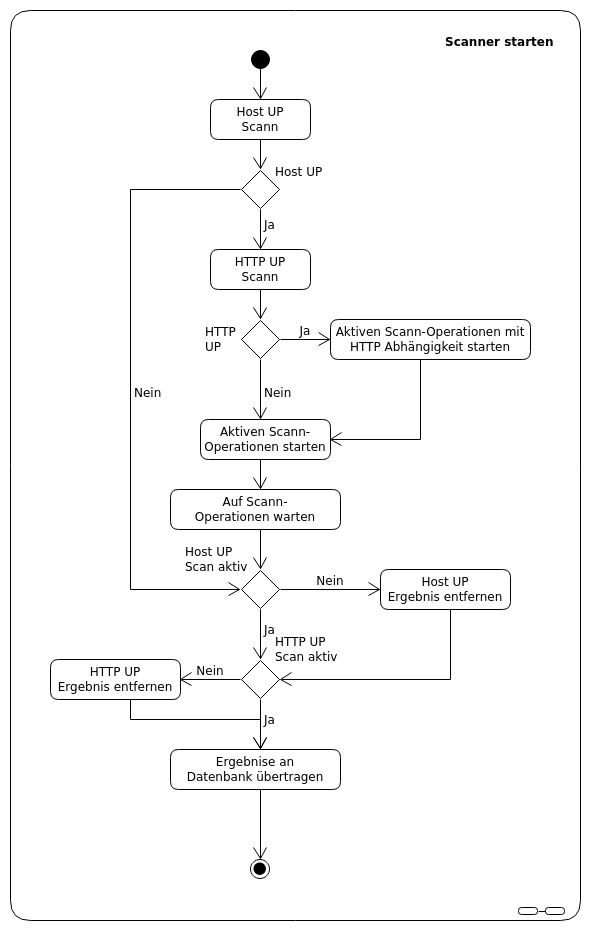
\includegraphics[width=\linewidth,height=\textheight,keepaspectratio]{entwurf/scanner/state_scanner_start}
	\captionof{figure}{Starten eines Scanners (Zustandsdiagramm)}
\end{center}

Beim Ausführen der Funktion \textit{start()} des Scanners wird zunächst geprüft, ob das entfernte System erreichbar ist. Sollte dies nicht der Fall sein, werden alle nachfolgenden Scan-Operationen nicht durchgeführt, da diese fehlschlagen würden. Im Anschluss wird getestet, ob der HTTP Dienst des entfernten Systems erreichbar ist, da dieser für einige weitere Tests benötigt wird. Ist der HTTP Dienst erreichbar, werden die Scan-Operationen, welche auf dem HTTP Dienst basieren, mit in die Liste der abzuarbeitenden Scan-Operationen aufgenommen. Danach werden alle verbleibenden Scan-Operationen nebenläufig gestartet. Nachdem die Scan-Operationen ihre Aufgabe abgeschlossen haben, sammelt der Scanner alle Ergebnisse ein. Falls die \textit{Host UP Scan-Operation} oder die \textit{HTTP UP Scan-Operation} deaktiviert ist, werden diese aus dem Ergebnis entfernt. Danach übermittelt der Scanner die gesammelten Ergebnisse zur Datenbank und beendet seine Scan-Runde.

\subsection{Scan-Operationen}

Die Scan-Operationen werden nebenläufig abgearbeitet, um so die Dauer eines kompletten Scans zu minimieren. Eine Scan-Operation prüft genau einen Dienst beziehungsweise eine Schwachstelle auf dem entfernten Rechner. Die im alten System implementieren Scans werden in die Scan-Operationen überführt. Deshalb sollen die folgenden Scan-Operationen implementiert werden.

\begin{itemize}
	\item Host-Up \\
	prüft, ob der entfernte Rechner mit Hilfe von ICMP Paketen erreichbar ist
	\item Bubble-Up \\
	prüft, ob der Bubble Server erreichbar ist und ob die Telnet Steuerung funktioniert
	\item BubbleNg-Up\\
	prüft, ob der Bubble NG Server erreichbar ist und ob die Telnet Steuerung funktioniert
	\item FTP-Save\\
	prüft, ob der FTP Server erreichbar und ob die Nutzung des anonymen Logins unterbunden worden ist
	\item Htaccess-Save\\
	prüft, ob die Kombination aus Nutzername und Passwort des Htaccess Schutzes geändert wurde
	\item SQL-Injection-Save\\
	prüft, ob die SQL-Injection im Login zum Membersbereich verhindert wurde
	\item SQL-Password-Save\\
	prüft, ob das lokale Passwort des SQL-Nutzers root geändert wurde
	\item Telnet-Save\\
	prüft, ob der Telnet Server deaktiviert oder deinstalliert wurde
	\item HTTP-UP\\
	prüft, ob der HTTP Dienst des entfernten Rechners nutzbar ist
	\item HTTPS-UP\\
	prüft, ob der HTTPS Dienst des entfernten Rechners nutzbar ist
	\item XSS-Save\\
	prüft, ob der Cross-Site-Scripting Angriff im Bewertungsformular behoben wurde.
\end{itemize}

\begin{center}
	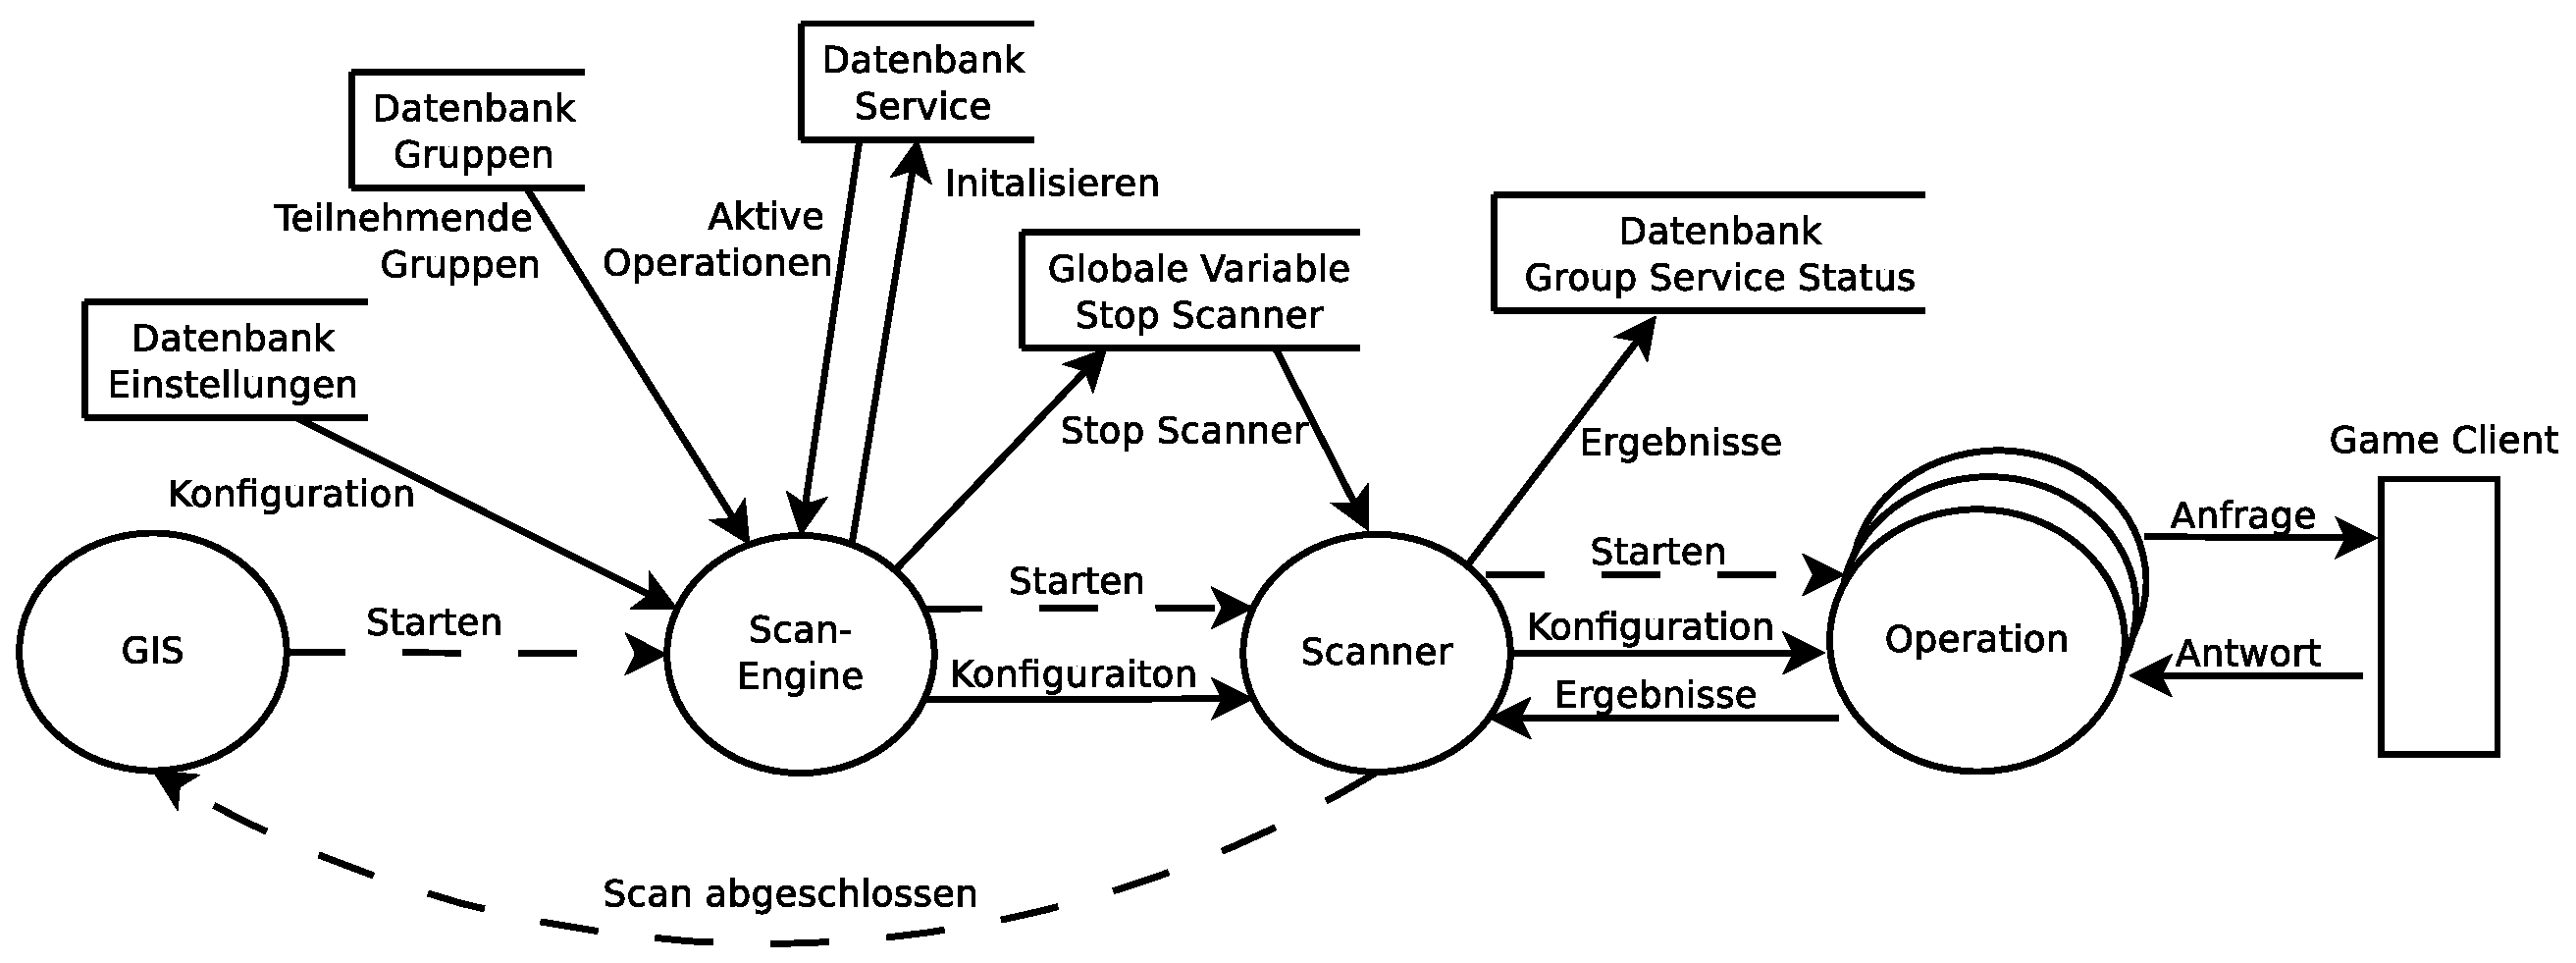
\includegraphics[width=\linewidth]{entwurf/scanner/dfd-scanner}
	\captionof{figure}{Datenfluss in der Scanner Komponente (Datenflussdiagramm)}
	\label{fig:dfd-scanner}
\end{center}

Die im Datenflussdiagramm (\autoref{fig:dfd-scanner}) sichtbaren, aber bisher nicht beschriebenen Datenflüsse finden zwischen dem Webserver und dem Scanner oder einer Scan-Operation und dem Game Client statt. Administratoren können über den Webserver den Scanner an- und abschalten. Die Scan-Operationen fragen bei dem Game Client ihren überwachten Dienst beziehungsweise ihre überwachte Schwachstelle an und erhalten eine Antwort zurück. Anhand dieser wird das Ergebnis der Scan-Operationen bestimmt.
	\section{Webserver} \label{sec:Webserver}
Der Webserver bietet die Möglichkeit der Verwaltung des Spiels, der Abgabe von Flags sowie der Durchführung von Käufen im Flagshop und Challenges. Auch können Informationen zum Spiel, wie Einstellungen, Spielstand, Strafen und Teilnehmer abgerufen werden.

\subsection{Verwendung mehrerer Microservices}
Der Webserver kann nach dem Architekturmuster Microservices implementiert werden. Hierbei besteht die Anwendung aus mehreren unabhängig Komponenten, welche, sofern dies notwendig ist, untereinander kommunizieren. Die Komponenten sind so klein wie möglich und können jederzeit durch eine andere Implementierung ausgetauscht werden. \cite{wolffMicroservicesGrundlagenFlexibler2015} 

So wären die verschiedenen Komponenten des Webservers (Flagabgabe, Nutzerverwaltung, Spielsteuerung, etc.) unabhängig von einander und können leichter weiterentwickelt oder ersetzt werden.

Die Verwendung dieses Architekturmuster würde bei der aktuellen Aufgabenstellung zu hohen Aufwand für zu wenig Nutzen bedeuten.

\subsection{Fat Webserver}
Der Webserver beinhaltet sowohl die Logik als auch die Darstellung. Bei einer Anfrage an den Webserver, wird eine Antwort bestimmt und diese dann in eine Vorlage / ein HTML Dokument eingebettet. Danach wird dieses zurück an den Nutzer gesendet.

Während der Implementierung des Prototyps und des weiteren Entwurfs hat sich ein Problem mit dem Flagshop Login herausgestellt.

Für die Nutzung des Flagshops ist ein Multi-Login notwendig, da nur am Webserver eingeloggte Nutzer sich mit einem extra angelegten Account am Flagshop anmelden und diesen verwenden dürfen. Dieses ließ sich mit dem im Prototypen implementierten Session basierten Login nicht einfach umsetzen. 

So ist für diesen Anwendungsfall ein Stateless Login besser geeignet, da hier die benötigten Informationen vom Client, je nach Anliegen, gesendet werden können. 

Die Nutzung des Stateless Logins bietet die Perspektive der Verwendung eines Stateless Webservers sowie eines Thin Webservers. Bei einem Thin Webserver werden nur Daten und keine Repräsentation an dem Client zurückgesendet. So wird die Aufgabe der Darstellung der Daten an den Client übertragen.

Durch die Nutzung eines Thin Servers werden zwei Dinge ermöglicht. 

Zum ersten ist es möglich den Client und Server unabhängig voneinander zu entwickeln, zu verändern und zu verbessern. Damit kann in Zukunft eine Iteration der Software einfacherer geschehen. Zweitens können die Studierenden eigene Clients programmieren, um mit der Anwendung zu interagieren.

\subsection{Thin Webserver}
\begin{center}
	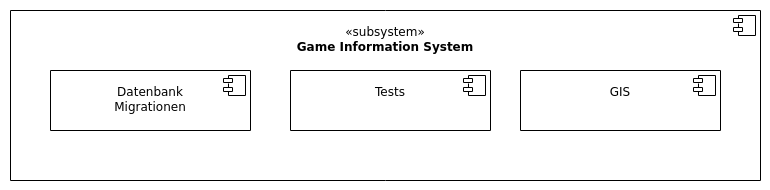
\includegraphics[width=\linewidth]{entwurf/gis/comp-gis}
	\captionof{figure}{REST Interface im Überblick (Komponentendiagramm)}
\end{center}

Der Server besteht aus der Komponente \textit{Game Information System}, welche wiederum aus drei weiteren Komponenten besteht. 

Die Komponente \textit{GIS} implementiert die gesamte Server Logik. In diesem Modul wird der eigentliche Thin Server, über das die Spieler und Betreuer mit der Anwendung interagieren können, implementiert.

In der Komponente Datenbank Migrationen sind Migrationsskripts hinterlegt, welche die Datenbank Iterationen festhalten. Diese Skripts sollen genutzt werden, um verwendete Datenbanken einfach auf den gleichen Soll-Zustand bringen zu können. 

Die letzte Komponente beinhaltet Unit-Tests. Mithilfe der implementierten Unit-Tests kann die Anwendung bei späteren Änderungen auf Fehler überprüft werden kann.


Da der Thin Server nur eine Brücke zwischen Nutzer und Scanner oder Datenbank darstellt, kann von einer API (Application-Programming-Interface) gesprochen werden. Mithilfe dieser API kann beispielsweise der aktuelle Spielstand aus der Datenbank ausgelesen und Strafen eingetragen werden.

\subsubsection{API}
Um bei der Implementierung der API einem Standard / einem Vorgehen zu folgen, wird der de facto Standard für HTTP-APIs Representational State Transfer (REST) verwendet.

Ein RESTful Interface ermöglicht, dass Ressourcen auf dem Webserver eindeutig identifizierbar sind, damit diese als Ziel von Operationen ausgewählt werden können. Des Weiteren werden einheitliche Schnittstellen genutzt. Dazu müssen Standardmethoden und -repräsentationen genutzt werden.

Durch diese Anforderungen biete das REST Interface die Möglichkeiten alle zur Verfügung stehenden Ressourcen auf die gleiche Art und Weise zu verwalten. Mit dieser Herangehensweise wird die HTTP Methode GET nicht länger zur Veränderung oder Erschaffung von Ressourcen verwendet, sondern die dafür ausgelegten HTTP-Methoden. Die für die Verwendung benötigten Daten werden auch nicht länger als Paramter der Anfrage beigefügt, sondern im Body der Anfrage übertragen. \cite{beimsWebApplikationenREST2014}

Alle Routen werden mit dem Präfix \textit{/v1} versehen, um bei späteren Iterationen der API Kollisionen zu verhindern und die Nutzung der API v1 weiterhin zu ermöglichen. 

Bei der Implementierung sollen die zur Verfügung stehenden HTTP Methoden benutzt werden. Das REST-Interface soll auch mit entsprechenden HTTP Codes antworten, um die Antwort und den Erfolg einer Anfrage auch ohne Antworttext interpretieren zu können. Bei der Datenübertragung zwischen Client und Server soll das JavaScript Object Notation (JSON) Format für die Formatierung der gesendeten Daten verwendet werden.

\begin{table}
	\centering
	\begin{tabular}{c c}
		GET & Auf Ressourcen zugreifen \\ 
		POST & Neue Ressourcen erzeugen \\  
		PUT & Bestehende Ressourcen verändern \\
		DELETE & Vorhandene Ressourcen löschen \\
	\end{tabular}
	\caption{Übersicht über die verwendeten HTTP Methoden}
	\label{table:http-methods}
\end{table}

Neben den in \autoref{table:http-methods} aufgezeigten Methoden gibt es noch weitere HTTP Methoden, welche keine Anwendung in dem zu implementierenden REST-Interface erhalten.

\subsection{Funktionale Eigenschaften}
(todo: Module / Komponenten des REST-Interface)
\paragraph{Authentifizierung}

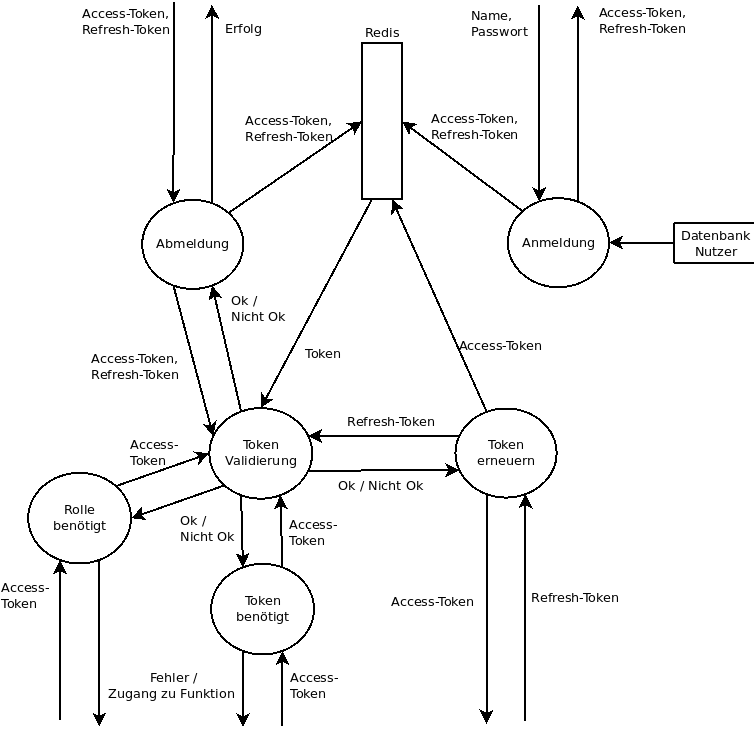
\includegraphics[width=\linewidth]{entwurf/gis/dfd-watchdog-security}
\captionof{figure}{Datenfluss in der Security Komponente (Datenflussdiagramm)}

\paragraph{Flaggengenierung}
- Änderung des Algo
- Änderung des Vorgehens -> Generierung auf dem Server -> Versand an den Client (Secret nicht auf dem Client, Abfangen aller Flags möglich, Verschlüsselung bringt nix, da Nutzer root Rechte hat)

\paragraph{Challenges}
todo:
Challenge Informationen und Lösung der Challenge über API, Darstellung / Inhalt der Challenge über anderen Webserver (da wo auch der Webclient ausgelieftert wird), da gedanke ist nur Daten zu übertragen und keine HTML Seiten etc.

\subsection{Reverse Proxy}
Für das Betreiben wird auf den bereits im EZS Labor verwendeten Apache HTTP-Server zurückgegriffen. Durch die Entscheidung bleibt dieser als einziger als Einstiegspunkt für Anfragen zuständig. Des Weiteren wird die Protokollierung der Anfragen sowie die Verschlüsselung der Verbindung an die Webserver Software abgegeben.

Der Reverse Proxy muss bei der Weiterleitung der Anfrage an das GIS die eigentliche IP-Adresse der Anfrage weiterleiten. Dieses wird benötigt um die IP-Adresse, und so die zugehörige Gruppe, bei der Registrierung und dem Login zu bestimmen. Die originale IP-Adresse der Anfrage soll in einen HTTP Header gespeichert werden.

In einen HTTP Header können Server und Client zusätzliche Informationen zur Anfrage oder Antwort beifügen. \cite{mdncontributorsHTTPHeaders2020}

Um einen Spoofing-Angriff zu erschweren und das Vertrauen in den Header mit der IP-Adresse zu erhöhen, soll ein weiterer Header mit einem Geheimnis gesetzt werden. Anhand dieses kann das GIS entscheiden, ob die Anfrage über einen vertrauenswürdigen Proxy weitergeleitet oder ob ein Spoofing-Angriff durchgeführt worden ist. Die Erweiterung wird benötigt, da die Anwendung auch ohne einen Reverse Proxy betrieben werden kann. In diesem Anwendungsfall kann die angreifende Person sich als Proxy für eine andere Gruppe ausgeben.

Bei einem Spoofing-Angriff versendet die angreifende Person Anfragen für andere IP-Adressen und erhält die Antwort. So kann dieser im Namen anderer agieren und diesen beispielsweise Minuspunkte verschaffen.
	\section{Datenbank}
- Daten in Verbindung setzen, keine redundanz
- Ordnung der Daten
- zentrale Speicherort
- Atomare Operation -> keine unvollständigen Daten
- Daten müssen erhalten bleiben
- Abfragen besser optimiert als auf Dateien
- Views zur Berechnung von Punkten

Daten haben Schema, Keine großen Datenmengen

-> relationale db

\subsection{ASDF-Tabellen}
Bild hier

In der Abbildung \ref{label} ist neben der alleinstehenden Tabelle \textbf{\textit{settings}} die Tabelle \textbf{\textit{users}} sowie die n zu m Beziehung zwischen \textbf{\textit{users}} und \textbf{\textit{groups}} dargestellt. Die n zum m Beziehung wird über eine Referenztabelle (\textbf{\textit{penalties}}) mit einer 1 zu n Beziehung zwischen \textbf{\textit{groups}} und \textbf{\textit{penalties}} und einer 0,1 zu n Beziehung zwischen \textbf{\textit{users}} und \textbf{\textit{penalties}} modelliert. In der n zu m Beziehung werden die ausgesprochen Strafen gespeichert. Jede Gruppe kann von mehreren Betreuern oder dem System mehrmals verwarnt werden.

\subsubsection{Einstellungen}
Die \textbf{\textit{settings}} Tabelle beinhaltet Einstellungen des Spiels als key-value Paar. Hierbei sind beide Spalten strings und der key einzigartig. Zu den Einstellungen gehört beispeilsweise das Scan-Intervall, die Flags pro Team sowie das Ende der Discover- und Attackzeit.

\subsubsection{Nutzer}
In der Tabelle \textbf{\textit{users}} sind die Log-In Informationen der Administratoren, Betreuer und Spieler hinterlegt. Da der Login aus Nutzername und Passwort besteht, werden die Spalten \textit{name} und \textit{password} benötigt. Auch muss anhand des Nutzernamens eindeutig auf einen Account geschlossen werden, deshalb ist die Spalte \textit{name} als unique gekennzeichnet. Die Rolle des Nutzers wird mithilfe eines Enums (\textit{role}) (Liste von benannten Werten) definiert.

\subsubsection{Strafen}
Die durch das System oder die Betreuer verteilten Strafen werden in der Tabelle \textbf{\textit{penalties}} gespeichert. Dazu wird neben dem Grund der Strafe (\textit{reason}), der Zeitpunkt der Bestrafung (\textit{timestamp}) auch die Anzahl an Strafpunkten (\textit{points}) festgehalten. Damit Gruppen von einem Betreuer öfters bestraft werden können, ist der Primärschlüssel des Eintrages die ID der Strafe.

\subsection{Gruppen-Tabellen}
Bild hier

Wie in Abbildung \ref{label} zusehen existiert zwischen der Tabelle \textbf{\textit{groups}} und \textbf{\textit{group\_members}} eine 1 zu n Beziehung. Dies bedeutete, dass eine Gruppe mehrere Mitglieder haben kann, aber jedes Mitglied nur genau in einer Gruppe vertreten sein kann.

\subsubsection{Gruppe}
In der Tabelle \textbf{\textit{groups}} werden alle teilnehmenden GameClients vermerkt. Jede Gruppe besitzt eine eindeutige \textit{ID} und einen eindeutigen \textit{Namen}. Der \textit{Name} der Gruppe repräsentiert die IP-Adresse des GameClients und ist nach Classless Internet Domain Routing Konvention (CIDR) abgelegt. Des Weiteren besitzt die \textbf{\textit{groups}} Tabelle die Spalte \textit{token}. In dieser wird der individuelle Token, welcher zur Flaggenerierung benötigt wird, abgespeichert. Dies ist nötig, damit der Server die selben Flags wie der GameClient generieren kann und die Betreuer die Richtigkeit verifizieren können.

\subsubsection{Gruppenmitglieder}
Die Tabelle \textbf{\textit{group\_members}} beinhaltet alle IP-Adressen, welche im Namen einer Gruppe agieren dürfen. Dafür wird die IP-Adresse im Feld \textit{alias\_ip} und die vertretende Gruppe als Referenz im Feld \textit{group\_id} gespeichert. Da das Feld \textit{alias\_ip} als Primärschlüssel verwendet wird, kann jede IP-Adresse nur genau eine Gruppe vertreten.

\subsection{Flags-Tabellen}
Bild hier

In der Abbildung \ref{label} erkennbar ist die 1 zu n Beziehung zwischen der Tabelle \textbf{\textit{groups}} und \textbf{\textit{flags}}. Dieses hat zur Folge, dass eine Gruppe mehrere Flags besitzen kann, jedoch eine Flag immer genau zu einer Gruppe gehört. In der Abbildung ist weiter die n zu m Beziehung zwischen \textbf{\textit{groups}} und \textbf{\textit{flags}} abgebildet. Diese wird in eine Verknüpfungstabelle namens \textbf{\textit{flags\_submitted}} mit zwei 1 zu n Beziehung zerlegt. Diese Tabelle enthält die abgegeben Flags.
 
\subsubsection{Flags}
Die während eines Spiels generierten und benötigten Flags werden in der Tabelle \textbf{\textit{flags}} abgelegt. Hierzu wird der Wert der Flag als string in der Spalte \textit{flag\_value} festgehalten. Neben diesem wird Nutzungsart unter Zuhilfenahme eines Enums und die Gruppenzugehörigkeit als Referenz gespeichert. Neben diesem wird in der Spalte \textit{already\_bought} als bool vermerkt, ob diese Flag bereits im Flagshop erworben wurden ist. Diese Spalte besitzt nur Relevanz für die dementsprechenden Flagshop Flags.

\subsubsection{Abgegebene Flags}
Die durch die Studierenden abgegeben Flags werden in der Tabelle \textbf{\textit{flags\_submitted}} eingetragen. Auch wird der Zeitpunkt der Abgabe mitgespeichert, um eventuelle Betrüge aufzudecken. Die Spalten \textit{group\_id} und \textit{flag\_value} bilden zusammen den Primärschlüssel. Dieses ermöglicht, dass jede Gruppe jede Flagge und das eine Gruppe die selbe Flagge nicht mehrfach abgeben kann

\subsection{Service-Tabellen}
Bild hier

In der Abbildung \ref{label} ist die \textbf{\textit{services}} Tabelle sowie die n zu m Beziehung zwischen \textbf{\textit{groups}} und \textbf{\textit{service}} zu sehen. Diese wird als Referenztabelle (\textbf{\textit{group\_service\_status}}) mit zwei 1 zu n Beziehungen dargestellt.

\subsubsection{Services}
In der \textbf{\textit{services}} Tabelle sind alle vom Big Brother überwachten Schwachstellen eingetragen. Jeder dieser Einträge besteht aus einer eindeutigen ID, dem internen Namen der Operation (\textit{name}), dem angezeigten Namen (\textit{public\_name}) und der Gewichtung des Dienstes im Gesamtergebnis (\textit{weight}). Auch kann die Überprüfung der Schwachstelle mithilfe dem bool-Wert \textit{active} an- oder abgeschaltete werden.

\subsubsection{Servicestatus der Gruppen}
In der Referenztabelle \textbf{\textit{group\_service\_status}} wird das Ergebnis der Überprüfung der Schwachstellen jeder Gruppe abgespeichert. Dazu wird für die Kombination aus Gruppe und Service ein Eintrag angelegt und die Anzahl der Scans in \textit{scan\_count} und die Anzahl der erfolgreichen Scans in \textit{online\_count} gespeichert. Des Weiteren wird der Zeitpunkt des letzten Scans in \textit{last\_scan} und der Erfolg des letzten Scans in \textit{was\_online} festgehalten. Erfolgreich bedeutet in diesem Kontext, dass die Studierenden die überwacht Schwachstelle ausgebessert und den überwachten Dienst online gehalten haben.

\subsection{Flagshop-Tabellen}
Die Abbildung \ref{label} stellt die 1 zu n Beziehung zwischen den Tabellen \textbf{\textit{groups}} und \textbf{\textit{flagshop\_user}} dar. Das heißt, dass jeder Gruppe mehrere Flagshop Benutzer zugehörig sein können, jeder Benutzer aber genau einer Gruppe angehört. Des Weiteren wird die n zu m Beziehung zwischen \textbf{\textit{groups}} und \textbf{\textit{flagshop\_packages}} als Referenztabelle (\textbf{\textit{groups\_bought\_flagshop\_packages}}) mit zwei 1 zu n Beziehungen dargestellt. Diese beinhaltet die gekauften Flagshop Pakete pro Team.

\subsubsection{Flagshop Nutzer}
Für die Nutzung des Flagshops müssen die Gruppen einen oder mehrere Flagshop Nutzer anlegen. Diese werden in der Tabelle \textbf{\textit{flagshop\_user}} abgelegt. Hierfür wird neben der erstellenden Gruppe (\textit{group\_id}) auch das Passwort (\textit{password}) und der Name (\textit{name})  abgespeichert. Der Primärschlüssel wird aus der Gruppe und dem Namen gebildet. So ist der Nutzername für die Gruppe eindeutig. Mehrere Gruppen können aber Nutzeraccounts mit demselben Namen anlegen.

\subsubsection{Flagshop Pakete}
Die Betreuer und Administratoren können Flagshop Pakete anlegen, welche durch Studierende kaufbar sind. Diese werden in der Tabelle \textbf{\textit{flagshop\_packages}} abgelegt und erhalten Informationen zum Preis (\textit{price}) und der Anzahl der erhaltenen Flags (\textit{flag\_count}). Auch kann ein Name für das Paket über das Feld \textit{name} angegeben werden.

\subsubsection{Gekaufte Flagshop Pakete}
Die durch die Gruppen gekauften Flagshop Pakete werden in der Tabelle \textbf{\textit{group\_bought\_flagshop\_packages}} abgespeichert. Auch wird im Feld \textit{price\_paid} der beim Kauf gezahlte Preis festgehalten, da die Studierenden den Preis eines Flagshop Paketes beim Kauf reduzieren können. Jedes Paket kann genau einmal von jeder Gruppe gekauft werden, da sich der Primärschlüssel aus Gruppe (\textit{group\_id}) und Paket (\textit{flagshop\_packages\_id}) zusammen setzt.

\subsection{Challenge-Tabellen}
Bild hier einfügen

In der Abbildung \ref{label} ist die \textbf{\textit{Challenge}} Tabelle und die n zum m Beziehung zwischen den Tabelle \textbf{\textit{groups}} und \textbf{\textit{challenges}} zusehen. Diese Beziehung ist als Verknüpfungstabelle (\textbf{\textit{group\_has\_challenges}}) mit zwei 1 zu n Beziehung realisiert.

\subsubsection{Challenges}
Die \textbf{\textit{challenges}} Tabelle beinhaltet alle Challenges, welche von den Studierenden gelöst werden können. Jede Challenge besitzt eine eindeutige ID. Neben dieser wird für jede Challenge ein Titel / Name in \textit{name}, ein Hinweis in \textit{hint}, das zum Lösen benötigte Passwort in \textit{password}, die Anzahl der Punkte in \textit{points} und der Pfad, über den die Challenge abgerufen werden kann, gespeichert.

\subsubsection{Gestartete / Abgeschlossene Challenges}
Alle angefangen und abgeschlossenen Challenges werden in der Tabelle \textbf{\textit{group\_has\_challenges}} abgespeichert. Es wird das Startdatum (\textit{started\_at}) der Challenge, den Status des Abschluss (\textit{solved}) und bei erfolgreicher Absolvierung der Challenge das Enddatum ((\textit{solved\_at})) gespeichert. Durch die Zusammensetzung des Primärschlüssel aus Challenge und Gruppe, kann jede Gruppe jede Challenge genau einmal starten und absolvieren.

\subsection{Weitere Tabellen}
Bild hier

Wie in Abbildung \ref{label} erkennbar besitzen die Tabellen keine Abhängigkeiten und Verbindungen zu anderen. Im Folgenden werden die Tabellen für die Logs, die Notizen und die alten Spielstände vorgestellt.

\subsubsection{Logs}
Um die Aktionen innerhalb der Anwendung nachverfolgen zu können, werden diese in die \textbf{\textit{logs}} Tabelle geschrieben. Jeder Eintrag besteht aus einer ID, einem Enum in dem der Typ der Aktion festgehalten wird (\textit{action}), einem Zeitpunkt (\textit{timestamp}) und dem Inhalt der Aktion \textit{data}. 

Innerhalb der \textbf{\textit{logs}} Tabelle werden nur die Aktionen des derzeitig aktiven Spiels gespeichert. Neben diesen werden auch noch die Aktionen des letzten Spiels in der Tabelle \textbf{\textit{logs\_old}} gespeichert. Sollte ein Spiel beendet werden, werden die Aktionen des alten Spiels mit den neuen Aktionen überschrieben.

\subsubsection{Notizen}
In der Tabelle \textbf{\textit{notes}} soll den Betreuern und Administratoren die Möglichkeit geboten werden Notizen und Hinweise zum Rahmen und Durchführung des Versuches zu geben. Diese Notizen können durch die Studierenden eingesehen werden. Dafür werden Titel und Inhalt jeweils in einem string gespeichert. Um einzelne Notizen abrufen zu können, erhalten diese eine eindeutige ID.

\subsubsection{Alte Spiele}
Die Tabelle \textbf{\textit{backups}} soll alle alten Spielstände speichern. Dazu wird jedem Backup eine eindeutige ID zugewiesen und der Zeitpunkt des Erstellens wird in \textit{created\_at} abgespeichert. Die Informationen zu einem Spiel sind im JSON Format in der Spalte \textit{data} abgelegt.
	\section{Webclient} \label{sec:Webclient}
In diesem Abschnitt wird zuerst auf den Unterschied zwischen Multi Page Applications uind Single Page Applications eingegangen, um eine Architektur für die neue Weboberfläche zu wählen. Im Anschluss wird das Design unter Zuhilfenahme von Mockups erläutert´

\subsection{SPA vs MPA} \label{subsec:SPA_vs_MPA}

\paragraph{Multi Page Applications} \label{para:Multi_Page_Applications}
Multi Page Application, kurz MPA, ist die klassische Architektur für Webanwendungen. Bei dieser Architektur wird für jeden Request (Anfrage) an den Webserver eine neue Seite inklusive Ressourcen wie Cascading Style Sheets (CSS)\footnote{Beinhalten Regeln für die Darstellung von unter anderem HTML-Dokumenten}, JavaScript und Bildern geladen. Dieses kann an einem Beispiel verdeutlicht werden.

Auf einer Shop-Seite befinden sich 10 Produkte inkl. Bild und Kurzbeschreibung. Wird ein Produkt ausgewählt, sendet der Client einen Request / eine Anfrage an den Webserver. Der Webserver antwortet mit allen Ressourcen (siehe oben), welche für das Produkt benötigt werden. Der Client stellt dann aus den Ressourcen die Ansicht dar und das Produkt inklusive der Details ist für den Nutzenden zu sehen.

Der Vorteil von MPAs ist die einfacherer Optimierbarkeit für Suchmaschinen, das sogenannte SEO (Search Engine Optimization). Ein gutes SEO Rating sorgt dafür, dass die Webseite bei Suchmaschinen weit oben zu finden ist. Dies ist besonders für Webseiten wichtig, die um Kunden konkurrieren. Anzuführen sind hier diverse Online-Shops und Zeitungen.

\paragraph{Single Page Applications} \label{para:Single_Page_Applications}
Die Single Page Application, kurz SPA, stellt das genaue Gegenteil von MPA dar. Bei SPAs besteht die Anwendung aus genau einem HTML-Dokument, dessen Inhalt bei Bedarf dynamisch nachgeladen wird. Dafür findet ein asynchroner Datenaustausch zwischen Client und Server statt, bei dem benötigte Ressourcen wie Bilder, JavaScript und CSS ausgetauscht werden. Durch dieses Verfahren wird sichergestellt, dass gleiche Elemente oder Ressourcen nicht erneut heruntergeladen werden müssen. Bei Änderungen werden nur Teile des DOMs\footnote{Das Document Object Model repräsentiert die Webseite als Baumstruktur} ersetzt und neu gerendert.

Die Interaktion mit dem DOM oder auch Virtual DOM kann selbst entwickelt werden. Jedoch ist hierbei zu raten, auf bereits bestehende Frameworks wie Angular (Entwickelt unter der Leitung vom Angular Team bei Google), React (Entwickelt unter der Leitung von Facebook) oder Vue (Evan You und Core Team) zurückzugreifen. 

Der große Vorteil von SPAs ist die Geschwindigkeit der Anwendung, da hier nur einzelne Teile ausgetauscht werden müssen. SPAs bieten außerdem den Vorteil, dass die Entwicklung von Front- und Backend entkoppelt wird. Das heißt, dass die Programmierenden des Front- und Backends weitestgehend unabhängig voneinander arbeiten können.

Die SEO-Optimierung gestaltet sich schwieriger, da es sich um eine dynamische Anwendung handelt. Zur Nutzung von SPAs muss im Browser JavaScript in der benötigten Version verfügbar und aktiviert sein.

\paragraph{Zusammenfassung Vor- und Nachteile} \label{para:Zusammenfassung_Vor-_und_Nachteile}
\mbox{} % Damit die Tablle in der neuen Zeile angezeigt wird
\begin{center}
	\begin{tabular}{rcc}
		& SPA & MPA \\
		Vorteile &
		\begin{minipage}[t]{0.4\textwidth}
			\begin{itemize}
				\item Sehr schnell, dank dynamischem Nachladen
				\item Entkoppelung zwischen Front- und Backend
				\item Effizientes cachen von Daten
			\end{itemize}
		\end{minipage} &
		\begin{minipage}[t]{0.4\textwidth}
			\begin{itemize}
				\item MPA Architektur ist ausgereift
				\item MPAs sind entwicklerfreundlich, da ein kleiner Technologiestack benötigt wird
				\item Ältere Browser werden in der Regel unterstützt
				\item SEO ist einfacher zu implementieren
			\end{itemize}
		\end{minipage}\\
		& & \\ % Space zwischen Vor- und Nachteilen
		Nachteile &
		\begin{minipage}[t]{0.4\textwidth}
			\begin{itemize}
				\item JavaScript muss in der benötigten Version im Browser verfügbar sein
				\item Alte Browser werden nur teilweise unterstützt
				\item Herausfordernde SEO Implementierung
			\end{itemize}
		\end{minipage} &
		\begin{minipage}[t]{0.4\textwidth}
			\begin{itemize}
				\item Anwendungen sind weniger performant als SPAs
				\item Front- und Backend haben eine starke Kopplung
			\end{itemize}
		\end{minipage}
	\end{tabular}
\caption{Vor- und Nachteile SPA/MPA}
\label{tab:Vor-_und_Nachteile_SPA/MPA}
\end{center}

Für die Entwicklung der Anwendung entscheide ich mich für die Verwendung einer SPA. Dies geschieht unter den Gesichtspunkten der Entkopplung zwischen Front- und Backend, der Performance der Anwendung und der Zukunftssicherheit, die meiner Meinung nach für SPAs besteht. Die Nachteile vom SPAs betreffen meine Anwendung nur wenig. So ist auf den Rechnern im Labor ein moderner Webbrowser installiert und in diesem JavaScript aktiviert. Auch handelt es sich um eine interne Anwendung, bei der die SEO Optimierung keine Rolle spielt. \cite{melnikSinglePageApplication2020}

\subsection{Mockups} \label{subsec:Mockup}

Für das Layout der Oberfläche wird die Designsprache Material Design von Google verwendet, da dieses konkrete Gestaltungsregeln vorgibt und einen Styleguide zur Verfügung stellt. Material Design wurde im Jahr 2014 vorgestellt und in Apps von Google verwendet. Besonders die Optimierung der Benutzerfreundlichkeit steht im Vordergrund. Eine Besonderheit des Material Designs ist, dass physikalische Gesetze beachtet werden und die Inhalte für eine Priorisierung auf einer virtuellen Z-Ebene verschoben werden. \cite{kulturbanause-teamMaterialDesignDesignsprache2017}

Den Prinzipien des Dark Theme von Material Design wird gefolgt, da die bestehende Anwendung bereits nur im Dark Mode vorhanden ist. Des Weiteren werden Anwendungen derzeitig häufig mit Dark Mode als Default Theme veröffentlicht und bestehende Anwendungen ohne Dark Mode erhalten diesen als zusätzliches Farbschema. \cite{colbyWindows10Dark2020}

Das Dark Themes trägt zur Verbesserung der visuellen Ergonomie bei, was zu einer Reduktion der Belastung der Augen führt. Des Weiteren wird bei OLED-Bildschirmen die Batterieleistung geschont. Die im Light Theme verwendete Verschiebung auf der Z-Ebene wird durch Schatten erreicht und ist deshalb im Dark Theme nicht nutzbar. Anstatt einer Verschiebung werden die Elemente unterschiedlich beleuchtet.\cite{googleDarkTheme}

Damit die Icons zum Design der Seite passen und Einheitlich sind, werden Material Design Icons\footnote{\url{https://materialdesignicons.com/}} verwendet. Hier sind die offiziellen Icons sowie Icons von der Community, die dem Material Design Ansatz folgen, vorhanden.

\begin{center}
	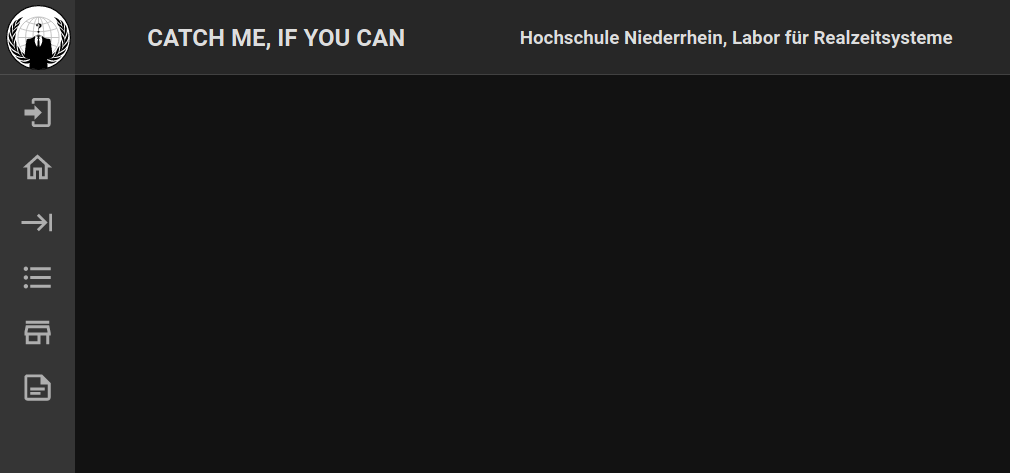
\includegraphics[width=\linewidth]{entwurf/webclient/base}
	\captionof{figure}{Grundlayout der Weboberfläche (Mockup)}
	\label{fig:mockup-base}
\end{center}

Das Grundlayout ist wie in \autoref{fig:mockup-base} abgebildet in drei Bereiche, Header (1), Navigation (2) und Content (3), eingeteilt. 

Der Bereich des Headers ist im oberen Teil erkennbar. Dort ist ein Logo, derzeitig noch das Logo aus der alten Anwendung, eine Überschrift sowie ein Untertitel platziert. Über die Überschrift und den Untertitel können die verschieden Seiten (Admin-, Spieler-, Flagshop- und Challengeseite) unterscheidbar gemacht werden.

Die Navigation ist auf der linken Seite erkennbar und als Sidebar mit Icons realisiert. Diese beinhaltet Verweise zu den Unterseiten. Sollte ein Eintrag der Navigation aktiv sein, wird dieser mithilfe der im Material Design vorgesehenen Farbe hervorgehoben.

Der Rest der Seite ist der Content Bereich. Dieser wird dynamisch mit dem anzuzeigenden Inhalt gefüllt.

\begin{center}
	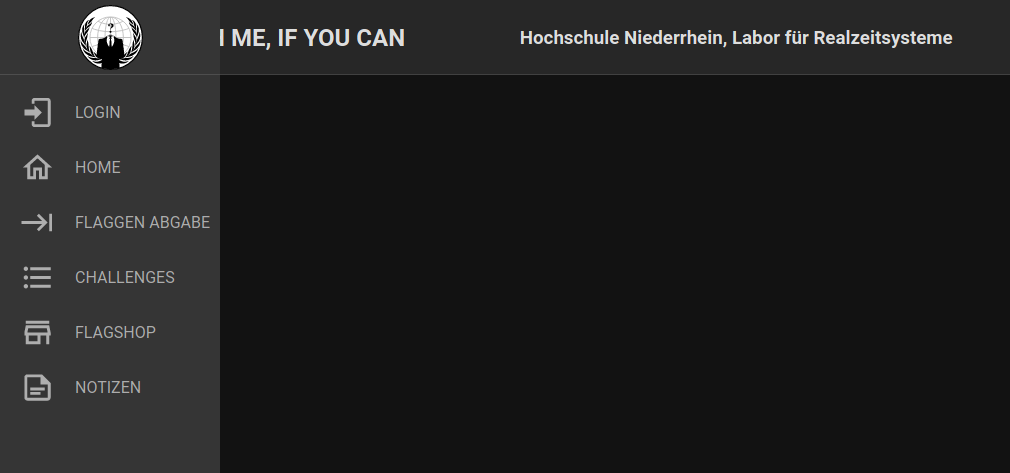
\includegraphics[width=\linewidth]{entwurf/webclient/base-extended}
	\captionof{figure}{Ausgeklapptes Menü beim drüberfahren (Mockup)}
	\label{fig:mockup-base-extended}
\end{center}

Damit die Navigation verständlich wird, gibt es wie in \autoref{fig:mockup-base-extended} zu erkennen neben den Icons auch beschreibenden Text. Dieser Text wird angezeigt, wenn der Nutzende mit der Maus über die Sidebar fährt. Die Sidebar wird über den Content ausgefahren und überdeckt diesen.

\begin{center}
	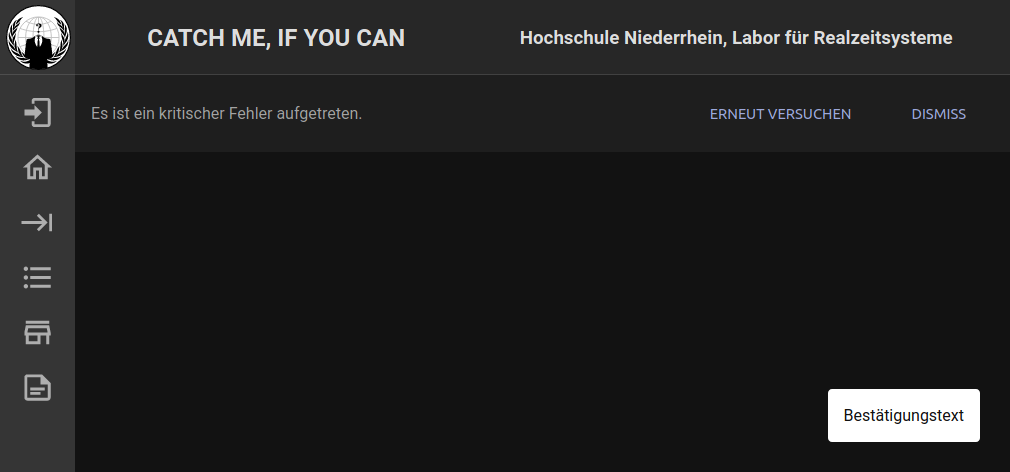
\includegraphics[width=\linewidth]{entwurf/webclient/base-with-error}
	\captionof{figure}{Fehlernachrichten (Mockup)}
	\label{fig:mockup-base-with-error}
\end{center}

Sollte der Nutzende über Ereignisse informiert werden, stehen zwei Möglichkeiten zur Verfügung.

Wenn das Ereignis wichtig ist, wird ein Banner verwendet. Dieser Banner besteht aus drei Elementen, einem Element für die Nachricht und zwei Buttons. Der linke der beiden ermöglicht es dem Nutzenden eine Aktion direkt auszuführen. Dies kann unter anderem eine Weiterleitung zu einer bestimmten Seite sein, über die der Nutzende weitere Informationen erhält. Über den anderen Button kann der Banner ausgeblendet werden. Es wird maximal ein Banner zeitgleich angezeigt.

Die andere Möglichkeit den Nutzenden zu informieren, ist die sogenannte Snackbar. Diese wird verwendet, wenn die Benutzererfahrung nicht unterbrochen werden soll und keine Benutzereingabe benötigt wird.
Die Snackbar wird am  unteren rechten Rand platziert und verschwindet im Gegensatz zum Banner nach einer definierten Zeit automatisch. Wenn möglich wird auch hier maximal eine Snackbar gleichzeitig verwendet.

\begin{center}
	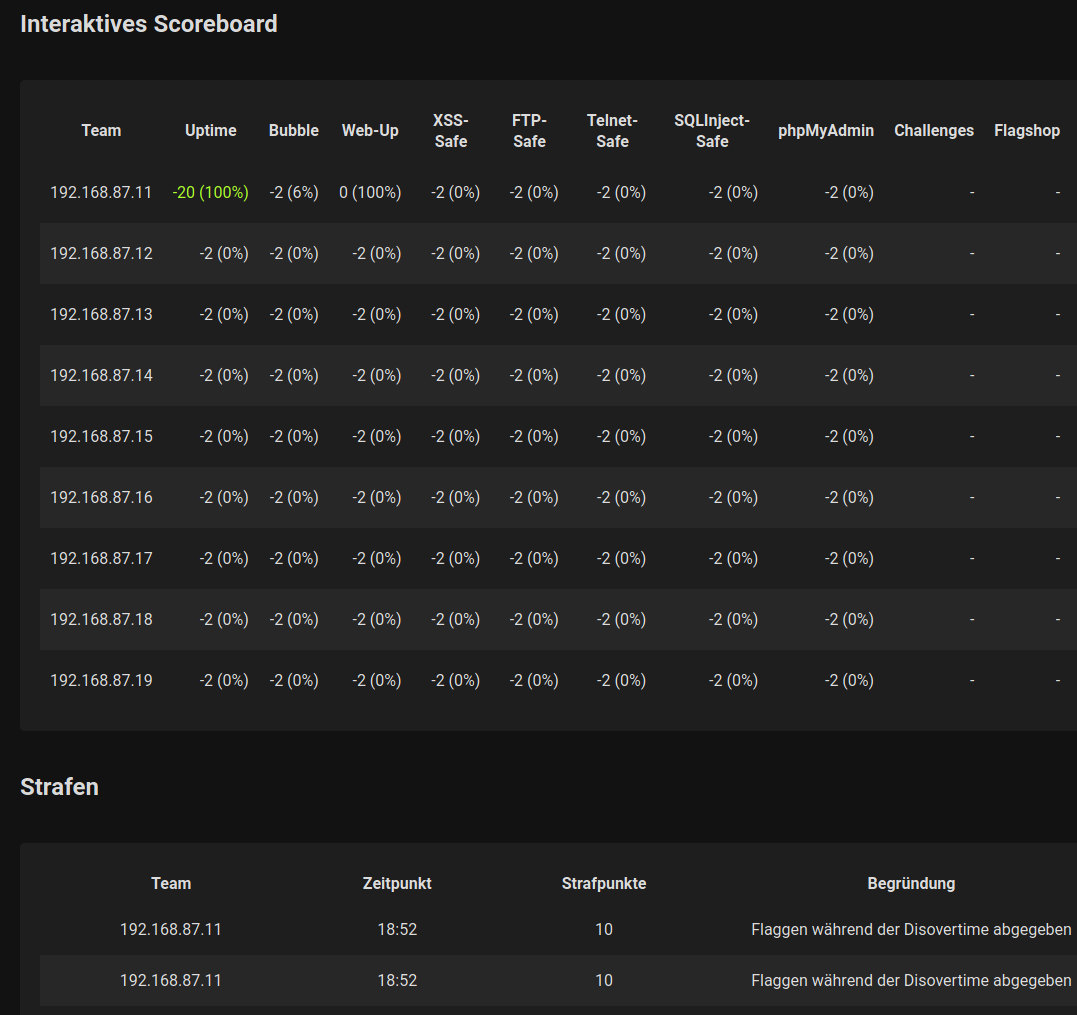
\includegraphics[width=\linewidth]{entwurf/webclient/table}
	\captionof{figure}{Ansicht des Spielstandes (Mockup)}
	\label{fig:mockup-table}
\end{center}

In \autoref{fig:mockup-table} ist ein Teil der Ansicht des Interaktiven Scoreboards inklusive der Strafen abgebildet. Die Ansicht ist in das Grundlayout der Anwendung (\autoref{fig:mockup-base}) eingebettet. Wie bereits oben erwähnt wird die Tabelle, um diese vom Hintergrund abzusetzen, unter Zuhilfenahme einer helleren Farbe dargestellt. Damit die Zeilen in der Tabelle besser erkennbar sind, ist jede zweite Zeile hervorgehoben. 

Dienste, die beim letzten Scan den gewünschten Zustand hatten, werden mit einem kontrastarmen grün dargestellt. Im Gegensatz zu der vorhanden Anwendung wird auf eine rote Darstellung der Dienste, bei unerwünschtem Zustand, verzichtet. Einzig die Gesamtpunkte werden im negativen Bereich rot dargestellt.

	\section{GameClient} \label{sec:GameClient}
Der GameClient bleibt durch diese Bachelorarbeit unberührt. Es ist jedoch eine Änderung an ihm vorzunehmen, damit er mit dem \textit{Game Information System} kompatibel ist.
Am Spiel können nur noch Gruppen teilnehmen, die ihre Teilnahme gegenüber dem GIS bekunden. Bei dieser Anmeldung erwartet das GIS einen Token, der bei der Generierung der Flags verwendet wird. 

In der derzeitig implementierten Startgame-Routine findet durch den GameClient keine \linebreak Bekundung der Teilnahme statt, somit wird auch kein Token übermittelt.

Auch muss die Hashfunktion zur Generierung an die im GIS verwendete Funktion angepasst werden, wenn nicht der auf dem GameClient verwendete \textit{MD5} Hash-Algorithmus implementiert ist. Dies ist notwendig, damit die generierten Flags vergleichbar bleiben.
	
	\chapter{Technologien}
	\label{chap:Technologien}
	\section{Backend} \label{sec:Backend}
Bei der Entwicklung des Webservers wird auf ein Backend-Webframework zurückgegriffen. Dieses erleichtert die Entwicklung und Wartung der Webanwendung in dem Werkzeuge und Bibliotheken zur Verfügung gestellt werden, welche allgemeine Aufgabe übernehmen. Zu diesen allgemeinen Aufgaben gehört das Verarbeiten von HTTP Anfragen, das Erstellen von HTTP Antworten und das Weiterleiten von Anfragen an die entsprechende Funktion. Bei der Implementierung der Logik müssen alle diese allgemeinen Aufgaben nicht mehr beachtet werden.

Um die Weiterentwicklung durch Studierende des Bachelor Informatik der Hochschule Niederrhein zu gewährleisten, werden nur Webframeworks, welche eine Programmierung in C, C++, Python oder JavaScript vorsehen, in Betracht gezogen. Da eben diese an der Hochschule Niederrhein gelehrt werden. Derzeitig sind neben Frameworks wie Spring (Java), Ruby on Rails (Ruby) und Laravel (PHP), welche nicht in den Vergleich aufgenommen werden, Django (Python), Flask(Python) und Express(Node.js/JavaScript) verbreitet.\cite{mdncontributorsServersideWebFrameworks2020}

In der Lehrveranstaltung \textit{Web-Engineering} wird die Entwicklung mehrere Backend-Server unter Zuhilfenahme von Python durchgeführt. Deshalb werden im folgenden nur Django und Flask betrachtet. 

Anschließend wird ein Framework gewählt, mit dem der Backend-Server realisiert werden soll.

\subsection{Django}\label{subsec:Django}
Django folgt der sogenannten \textit{Batteries Included} Philosophie. 

Bei dieser werden vielseitige Standardbibliotheken mit ausgeliefert, so dass ein Nutzer keine oder wenige separate Pakete herunterladen muss.\cite{kuchlingPEP206Python}

Django liefert unter anderem Modulen für Caching, Logging, Versenden von E-Mails, RSS-Feeds, Pagination, Security und der automatischen Generierung von Administrationsseiten. \cite{djangoDjangoDocumentationDjango} Durch den \textit{Batteries Included} Ansatzes funktionieren die Komponenten reibungslos untereinander und sind mit dem Kern kompatibel. Des Weiteren sind die Dokumentationen der verschiedenen Module zentrale an einem Ort verfügbar. 

Django wurde von einem Team entwickelt, welches ursprünglich Zeitungs-Websites erstellt und verwaltet hat. Dieses Team hat die gemeinsame Codebasis abstrahiert und in ein Framework überführt. Daher ist Django besonders, aber nicht nur, für Nachrichtenseiten und Content Managment Systeme (CMS) geeignet. \cite{mdncontributorsDjangoIntroduction2019}

\subsection{Flask}
Im Gegensatz zu Django ist Flask ein Mikroframework und verfolgt die \textit{Batteries Included} Philosophie nicht. Bei einem Mikroframework ist der Kern einfach, aber erweiterbar gestaltet und es gibt wenige bis keine Abhängigkeiten zu externen Bibliotheken. Dieser Ansatz überträgt der programmierenden Person mehr Verantwortung aber auch mehr Freiheiten. So trifft Flask beispielsweise nicht die Entscheidung, welche Datenbank genutzt werden soll. \cite{palletsForewordFlaskDocumentation2010} 

Wie bei Django (\ref{subsec:Django}) werden zwei Module bei der Installation von Flask mit geladen. Zum einen wird auf das Modul \textit{Werkzeug} zurückgegriffen, um eine ordnungsgemäße WSGI-Anwendung zu ermöglichen. Zum anderen wird Jinja2 mitgeliefert, da die meisten Anwendungen eine Template-Engine benötigen.
Flask will ein solide Grundlage für alle Anwendung sein, bei der die entwickelnde Person viele Freiheiten genießt.\cite{palletsDesignDecisionsFlask2010}

\subsection{Wahl des Frameworks}

Das Mikroframework Flask wird zur Implementierung des Webservers genutzt. Die Anwendung wird in Python geschrieben und kann daher durch Studierende weiterentwickelt werden, ohne dass diese sich in eine neue Programmiersprache einarbeiten müssen. Des Weiteren werden viele Module von Django nicht benötigt. Diese stellen einen Overhead dar. Auch handelt es sich bei der zu entwickelnden Software um eine vergleichbar kleine Anwendung. Es würden nur wenige Vorteile von Django genutzt. Flask kann mit Hilfe von Community Modulen bei Bedarf erweitert werden.
	\section{Datenhaltung} \label{sec:Datenhaltung}
Es gibt eine Vielzahl von verschiedenen relationalen Datenbankmanagementsystemen, die alle einen ähnlichen Funktionsumfang mitbringen.

Im Folgenden werden nur die kostenlos nutzbaren und am weitesten verbreiteten Datenbanken dargestellt. Zu dieser Liste zählen MySQL (Oracle), PostgreSQL (PostgreSQL Global Development Group), MariaDB (MariaDB Foundation) und SQLite (Dwayne Richard Hipp). \cite{db-enginesDBEnginesRanking}

Im Anschluss an die Darstellung wird die Wahl der Datenbank für die Anwendung begründet.

\subsection{MySQL und MariaDB}
MySQL ist das beliebteste Open-Source SQL Datenbankmanagementsystem, das im Jahr 1995 veröffentlicht worden ist. Dieses ist als Client/Server Architektur implementiert, kann aber auch in eingebetteten Systemen verwendet werden. \cite{oraclecorporationMySQLMySQLReference2020} MySQL ist in C / C++ geschrieben und kompatibel mit vielen Programmiersprachen, darunter auch Python. Des Weiteren ist es auf diversen Plattformen einsetzbar und für große Datenmengen optimiert. \cite{oraclecorporationMySQLMySQLReference2020a}

MariaDB ist eine Abspaltung von MySQL. Sie resultierte aus der bevorstehenden Übernahme von MySQL durch Sun Microsystems unter der Führung von Oracle. \cite{ionosMariaDBVsMySQL2020}

\subsection{PostgreSQL}
PostgreSQL ist frei verfügbar und ohne Lizenzierung nutzbar. Es wurde als universitäres Projekt an der University of California at Berkeley Computer Science Department gestartet. Es sind neben den SQL92 und SQL99 Standard auch einige eigene Erweiterungen implementiert. \cite{boenigkWasIstPostgreSQL} 

Nach Angaben der Entwickler ist \textquote[\cite{thepostgresqlglobaldevelopmentgroupPostgreSQLDocumentation122020}]{PostgreSQL [...] heute die fortschrittlichste Open-Source-Datenbank, die es gibt.} 

\subsection{SQLite}
Im Gegensatz zu den bereits vorgestellten Datenbanken handelt es sich bei SQLite um eine serverlose Datenbank, die nicht aufgesetzt oder verwaltet werden muss. SQLite speichert die Daten in einer gewöhnlichen Datei, welche kopiert und verteilt werden kann. \cite{sqliteFeaturesSQLite}

\subsection{Wahl der Datenbanksoftware}
Die PostgreSQL Datenbank wird den Alternativen vorgezogen, da es für den Anwendungsfall keine nennenswerten Unterschiede zwischen den Datenbanken gibt. Die erhöhte Komplexität von PostgreSQL im Vergleich zu SQLite kann durch die Nutzung eines Dockerimages reduziert werden. Des Weiteren haben sich die Studierenden mit der PostgreSQL Datenbank in der Veranstaltung \textit{Datenbanksysteme} beschäftigt und im EZS-Labor besitzen bereits Mitarbeiter Kenntnisse von PostgreSQL.
	\section{Frontend} \label{sec:Frontend}
Für die Realisierung des Frontends sollte aus den in Kapitel \ref{chap:Entwurf} auf ein bestehendes Framework zurückgegriffen werden. In der Betrachtung werden die drei beliebtesten JavaScript Frameworks, laut einer Stackoverflow (Frage- und Antwortseite für Programmierende) Umfrage, diskutiert. Die Umfrage, bei der circa 65.000 Menschen teilgenommen haben, wurde im Februar 2020 durchgeführt.\cite{stackexchangeStackOverflowDeveloper2020}

\begin{center}
	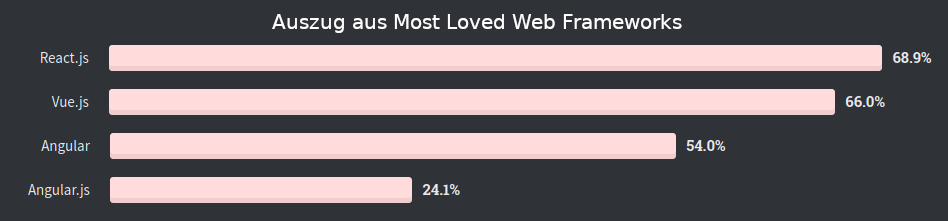
\includegraphics[width=\linewidth, keepaspectratio]{technologie/so-loved-fw}
	\captionof{figure}{Weiterverwendung des benutzten Webframeworks (Screenshot) \cite{stackexchangeStackOverflowDeveloper2020}}
	\label{fig:frontend-so-loved}
\end{center}

\begin{center}
	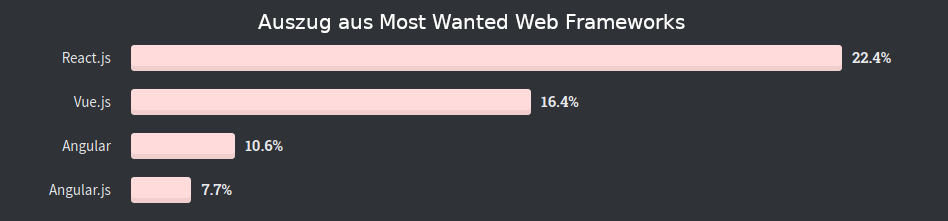
\includegraphics[width=\linewidth, keepaspectratio]{technologie/so-wanted-fw}
	\captionof{figure}{Interesse an einem neuen Webframework (Screenshot) \cite{stackexchangeStackOverflowDeveloper2020}}
	\label{fig:frontend-so-wanted}
\end{center}

In der Abbildung \ref{fig:frontend-so-loved} ist zu sehen, wie viele Prozent der Entwickelnden, welche bereits mit der Technologie arbeiten, ein Interesse bekundet haben diese für weitere Projekte zu nutzen. React.js führt diese Liste mit 69 \% an. Darauf folgt Vue.js dicht mit 66 \%. Bei Angular sieht dieses etwas anders aus, hier bekunden nur 54 \% ein Interesse. Im Gegensatz dazu wollen $\sim$25 \% der Befragten den Vorgänger Angular.js weiter nutzen.

Die Abbildung \ref{fig:frontend-so-wanted} zeigt in Prozent, wie viele Entwickelnden ein Interesse an der Technologie haben, bisher aber noch nicht mit dieser gearbeitet haben. Auch hier ist React.js mit $\sim$22 \% führend. Etwas abgeschlagen mit $\sim$16 \% folgt Vue.js. Dahinter reihen sich Angular mit $\sim$11 \% und Angular.js mit 8 \% ein.

\begin{center}
	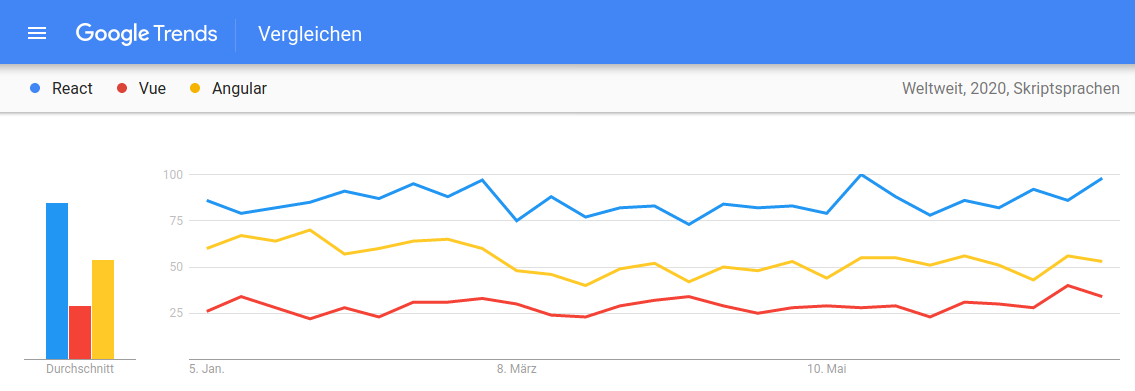
\includegraphics[width=\linewidth, keepaspectratio]{technologie/google-trends}
	\captionof{figure}{Google Trends (Screenshot) \cite{googleGoogleTrends2020}}
	\label{fig:frontend-google-trends}
\end{center}

\begin{center}
	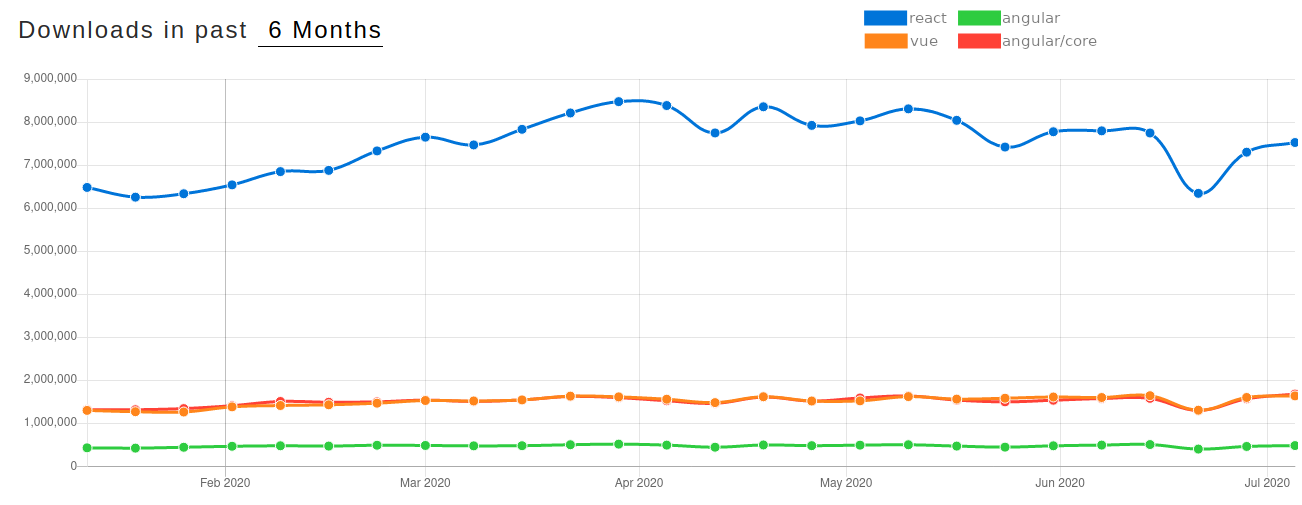
\includegraphics[width=\linewidth, keepaspectratio]{technologie/npm-trends}
	\captionof{figure}{NPM Trends (Screenshot) \cite{potterReactVsVue2020}}
	\label{fig:frontend-npm-trends}
\end{center}

Die Google Trends in Abbildung \ref{fig:frontend-google-trends} zeigen das normalisierte Interesse an einem Begriff vom Januar 2020 bis Anfang Juli 2020. Das Interesse wird von Google stichpunktartig anhand von Google Suchanfragen bestimmt. \cite{googleHaufigGestellteFragen2020}

In der Abbildung \ref{fig:frontend-npm-trends} werden die wöchentlichen Downloads pro Framework grafisch dargestellt. In dieser ist erkennbar, dass Vue.js und Angular ungefähr gleich oft heruntergeladen werden. Generell ist eine Stagnation der Frameworks erkennbar, einzig bei React.js schwanken die Downloadzahlen zwischen 6,5 und 8,5 Millionen. Derzeitig scheinen sich die Downloads bei ungefähr 7 Millionen pro Woche eingependelt zu haben.

Durch die Abbildungen \ref{fig:frontend-so-loved}, \ref{fig:frontend-google-trends} und \ref{fig:frontend-npm-trends} lässt sich schlussfolgern, dass React.js derzeitig das beliebteste und auch verbreitetest Framework ist. Das unbeliebteste Framework der Auswahl scheint Angular.js zu sein. Anhand der Grafiken fällt eine klare Positionierung von Vue.js und Angular zwischen React und Angular.js schwer.

Im Folgenden sollen die Frameworks genauer betrachtet werden, um eine Nutzung unter anderem anhand des Funktionsumfangs, der Mächtigkeit sowie der Komplexität zu beurteilen.

\subsection{Angular}
AngularJS wurde von einem Google Mitarbeiter (Misko Hevery) als Seitenprojekt gestartet. Das Nebenprojekt wollte er nutzen, um interne Webanwendungen einfacher zu entwickeln. Nachdem einige interne Anwendungen mit diesem Projekt erstellt worden sind, wurde AngularJS im Jahr 2010 als Open-Source-Projekt veröffentlicht. Es fand sowohl in Unternehmensprojekten als auch in Projekten der Open-Source Community Anwendung.

Einige Jahr nach der Veröffentlichung, begann sich die Landschaft der Webentwicklung durch Neuerungen und veränderten Standards in JavaScript zu verändern. Neben dieser Veränderung ist das Team an die Grenzen gestoßen, welches die Verbesserung des Frameworks anging. Dieses führte dazu, dass AngularJS über die Zeit an Modernität verlor.

AngularJS war beim Entwurf nie für Mobile oder Unternehmensanwendungen gedacht.
So entschied sich das Team bei Google mit der Entwicklung der Version 2 einen Neuanfang zu wagen und Angular 2 für solche Anwendungsfelder zu entwerfen.

Um Verwirrungen zu vermeiden, wurde das bis dahin bekannte Angular in AngularJS umbenannt und die neue Version Angular 2 genannt. Des Weiteren folgt die Versionierung von Angular seit Version 2 dem Semantic Versioning Prinzip bei dem die Versionsnummer in \textquote[\cite{preston-wernerSemanticVersioning}]{MAJOR.MINOR.PATCH} untergliedert wird. 

In der Anfangsphase von Angular 2 war es umständlich ein neues Projekt anzulegen, die Build-Größen waren vergleichsweise groß. So erarbeitete sich den Ruf sperrig zu sein.
Neben diesem wurde in Version 2 die Sprache von JavaScript zu TypeScript(Obermenge von JavaScript) umgestellt, welches andere Syntaxen und neue Konzepte zur Folge hatte. \cite{gaviganHistoryAngular2018}

Am 24.06.2020 erschien Angular2 in der Version 10.0.0 \cite{googleAngularAngularVersioning2020} und zählt wie bereits vorher dargestellt zu den beliebtesten Frontend-Frameworks.

Im Folgenden wird nur das aktuell beworbene Angular2 dargestellt und Angular genannt.

Bei der Entwicklung von Angular wurde auf Konsistenz, Produktivität, Wartbarkeit, Modularität und frühzeitige Fehlererkennung gesetzt.

Angular 2 basiert auf Komponenten und Diensten, welche alle identische Strukturen besitzen. Auch gibt Angular vor, wie wiederverwendbarer Code angelegt wird, sodass hierfür keine Code Styles notwendig sind. Des Weiteren erhält die Angular Dokumentation einen Style-Guide. So müssen die Unternehmen keinen eigenen Style-Guide erstellen, was eine Zeitersparnis darstellt.
Durch diesen konsistenten Aufbau wird auch eine bessere Wartbarkeit gewährleistet.

Durch die Konsistenz, die gegeben Style-Guides und den wiederverwendbaren Code steigt die Produktivität. Da die Entwickelnden eingeschränkter sind und nicht überlegen und bewerten müsse, ob das aktuell angewandte Vorgehen richtig ist. 

Die Wartbarkeit der geschrieben Anwendung profitiert von der Konsistenz und den Style Guides, da so jeder der Involviert ist, den Code leichter nachvollziehen und verändern kann. Die Wartbarkeit des Frameworks ist derzeitig durch das große Interesse der Community sowie der internen Nutzung bei Google gesichert.

Bei Angular wird der Code in Module organisiert. Durch die Nutzung dieses modularen Systems können diverse Teams an ein und derselben Anwendung arbeiten, ohne sich gegenseitig zu behindern.

Die frühzeitige Fehlererkennung wird durch die Nutzung von TypeScript ermöglicht. TypeScript biete im Gegensatz zu JavaScript Unterstützung für Typen. Die Nutzung der Typen ist in TypeScript nicht vorgeschrieben, aber dringend zur Fehlererkennung empfohlen.
Des Weiteren ermöglicht das Angular-CLI eine einfache Methode um Unittests und End-zu-End-Tests durchzuführen, so können Fehler entdeckt und behoben werden. \cite{wahlinWesentlichenVorteileAngular2017}

Diese Vorgaben führen zwar zu einer besseren Wartbarkeit und einer konsistenten Anwendung, schränken aber zeitgleich Entwickler ein. Um eine konsistene Anwendung zu erhalten, ist das Gerüst unflexibel.

Da Angular in Unternehmensanwendung verwendet werden soll, ist es Komplex und benötigt so eine gewisse Einarbeitungszeit. Diese steile Lernkurve muss durch neue Programmiere bewältigt werden.\cite{ventzkemediaAngularVsReact2018}

\subsection{React}
Im Jahr 2010 startete React als Port von XHP (PHP-Erweiterung, welche XSS Angriffe vorbeugen sollte) bei Facebook. Da XHP Probleme mit dynamischen Webanwendungen nicht löste, bat ein Facebook Software-Engineer um Zeit, damit er XHP unter zur Hilfenahme von JavaScript in den Browser bringen könne. \cite{dawsonJavaScriptHistoryHow2014}

Anfänglich wurde React noch unter \textquote{BSD  + patents} lizenziert. Diese Lizenz gewährte eine Nutzungslizenz und eine Patentlizenz, solange von einer Klage gegen Facebook bei möglichen Patentverletzungen abgesehen wird. Am 25 September 2017 wurde die Lizenz nach Kritik zu \textquote{MIT} gewechselt. \cite{kripalaniIfYouRe2017}\cite{larsonFacebookJustChanged2017} Die MIT-Lizenz ist eine sehr restriktiv arme Lizenz und gibt die Erlaubnis zur Veränderung, Modifikation und Nutzung ohne Kosten. Des Weiteren beinhaltet diese keine Copyleft. Bei einem Copyleft muss das Ergebnis der Entwicklung, welches die Software mit Copyleft nutzt, unter derselben Lizenz angeboten werden.\cite{wehnerSoftwareUnterMIT2020}

React besteht aus Komponenten und nutzt eine Syntaxerweiterung von JavaScript namens JSX um JavaScript und HTML zusammenzuführen. Die JSX-Datien müssen vor der Ausliferungen an den Client in JavaScript transformiert werden. Reacts Komponenten sollten möglichst klein sein und nur eine Aufgabe erledigen. Diese führt zu einer besseren Test- und Wartbarkeit sowie einem besseren Verständnis der Anwendung.

Auch nutzt React einen sogenannten Virtual DOM (Document Object Model). Die Nutzung des vDOM ermöglicht es Anwendungen auf dem Server zu rendern. Neben diesem können Unterschiede zwischen DOM und vDOM erkannt werden. Dadurch muss nicht mehr die gesamte Seite sondern nur die veränderte Komponente neu gerendert werden. Dieses führt zu einer besseren Performance. \cite{bezJavaScriptEinfuehrungReact2015}

Um Beispielsweise eine SPA Anwendung in React zu entwickeln muss auf Drittanbieter Anwendungen zurückgegriffen werden oder die entsprechenden Funktionen müssen selber programmiert werden, da diese nicht in React enthalten sind. Dieses stellt entweder Zeitaufwand oder Abhängigkeiten von weiteren Entwicklern dar.

\subsection{Vue}
Vue.js wurde durch einen damaligen Mitarbeiter von Google (Evan You) entworfen und entwickelt, nachdem er viele mit Angular gearbeitete hatte. Er wollte nur einen ganz kleinen Teil aus Angular nutzen. So begann er zunächst nur für sich, veröffentlichte aber im Februar 2014 Version 1.0.0 auf GitHub.

Das Projekt gewann auf GitHub Beliebtheit und die Community beteiligte sich. Die ersten Plugins wurden erschaffen und es bildete sich ein Core Team.

Vue liefert im Gegensatz zu den anderen vorgestellten Frontend-Frameworks nur das Data Binding und die Möglichekit Komponenten zu programmieren im Kern mit. Zusätzlich benötigte Funktionen können bei Bedarf als Module geladen werden. Dies macht Vue zu einem spezialisierten aber auch universell nutzbaren Framework. Es ist nicht so universell nutzbar wie Angular aber auch nicht so spezialisiert wie React.\cite{teufelVueJsTutorial2018}

Die Dokumentation von Vue ist leicht verständlich und die Community hilft schnell bei Fragen. 
Anwendungen in Vue sind in eine hierarchische Struktur von kleinen Komponenten untergliedert. Dies soll es ermöglichen, dass die Komponenten und so das gesamte System besser zu verstehen ist. Redundanz ist dort zulässig, wo diese benötigt wird.
Komponenten erhalten neben dem reinen HTML auch CSS und JavaScript und sollen atomar sein. Das heißt, dass diese alleine und ohne Bindungen zu einer Komponente in einer höheren liegenden Ebenen (logisch gesehen) nutzbar sind. Durch diesen Ansatz ist die Software übersichtlicher, was zu einer besseren Test- und Wartbarkeit führt.

Damit diese Trennung nicht nur in der Software, sondern auch auf der Dateiebene passiert, nutzt Vue hierfür die sogenannten Single File Components. Diese Dateien enden mit der Dateiendung \textit{.vue} und sind erst nach einer \textquote{Kompilierung} nutzbar. Eine Single File Component trennt HTML, CSS und JavaScript auf, sodass dieses übersichtlich betrachtete werden kann. \cite{teufelVueJsTutorial2018a}

Ein Nachteil von Vue ist, dass es von keiner großen Firma entwickelt/unterstützt wird, welche die Entwicklung vorantreibt und die Verbreitung erhöht. Des Weiteren werden Angular und React intern selber genutzt, sodass das Framework eine langfristige Nutzung hat. Aber seit circa 2016 nutzen immer mehr Unternehmen Vue. Hier sind beispielsweise GitLab (2016, \cite{schatzWhyWeChose2016}), Laravel und Nintendo zu nennen.\cite{techuzTopWebsitesBuilt2018}

\subsection{Wahl des Frontend-Frameworks}

Für das Frontend sollte entweder Vue oder React genutzt werden, da diese Einsteigerfreundlicher sind. Angular wird auf Grund der Komplexität und des Umfangs des zuschreibenden Frontends nicht in Betracht gezogen. Sowohl für Vue als auch für React sprechen ausreichend Gründe. 

Vue ist schlanker und noch etwas leichter zu erlernen als React, da hier nur Kenntnisse in JavaScript, CSS und HTML benötigt werden. Bei React werden noch Kenntnisse in JSX benötigt.

Für React spricht die Verbreitung und damit größere Community, welche bei Problemen konsultiert werden kann. Auch ist es wahrscheinlicher das Problemstellungen bereits auf Frage-Antwort Plattformen wie StackOverflow behandelt worden sind. 

Schlussfolgernd sollte für das Frontend React genutzt werden, da hier eine größere Community bei Fragen zur Verfügung steht.



	
	\chapter{Realisierung}
	\label{chap:Realisierung}
	%\input{60-Realisierung/xyz}
	
	\chapter{Zusammenfassung \& Aussicht}
	% Dummy client hinzufügen -> bool in der gruppen liste, wenn bool gesetzt ist wird der client nicht gescannt & sperat im UI angezeigt
	% Flask Restful ->  Request Parser durch bspw. Marshmallow LINK tausen, da er ab Version 2.0.0 deprecated ist, derzeitige version 0.3.8
	% Lokale Webseite auf Clients dem neunen Design anpassen.
	% Überlegen, ob der Token nicht durch den Server generiert werden sollte und dem Client mitgeteilt wird
	%\input{70-Ende/xyz}
	
	% Nachspann einleiten:
	\backmatter 
	% Einstellungen für die Fußzeile aktualisieren
	% 	Einstellungen nur für die rechten Seiten
	% 	Layout: Abschnitt  |  Seite
	\rofoot[\textbf{$\mid$~~\pagemark}]{\textbf{$\mid$~~\pagemark}}
	%	Einstellungen nur für die linken Seiten
	%	Layout: Seite  |  Kapitel
	\lefoot[\textbf{\pagemark~~$\mid$}]{\textbf{\pagemark~~$\mid$}}
	\chapter{Anhang}
	\begin{table}
	\centering
	\begin{tabular}{l l c c c c}
		Methode & Route	& Admin & Supervisor & Player  & Flagshop \\ [0.5ex]
		\hline &&&&&\\
		GET		& /									& $\surd$ & $\surd$ & $\surd$ & $\surd$ \\
		GET		& /associate 						& $\surd$ & $\surd$ & $\chi$ & $\chi$ \\
		POST	& /associate						& $\surd$ & $\surd$ & $\surd$ & $\chi$ \\
		DELETE	& /associate/<int:associate\_id>	& $\surd$ & $\surd$ & $\surd$ & $\chi$ \\
		POST	& /auth/flagshop/login				& $\chi$ & $\chi$ & $\surd$ & $\chi$ \\
		POST	& /auth/login						& $\surd$ & $\surd$ & $\surd$ & $\surd$ \\
		POST	& /auth/refresh						& $\surd$ & $\surd$ & $\surd$ & $\chi$ \\
		DELETE	& /auth/revoke/access				& $\surd$ & $\surd$ & $\surd$ & $\chi$ \\
		DELETE	& /auth/revoke/refresh				& $\surd$ & $\surd$ & $\surd$ & $\chi$ \\
		GET		& /backup							& $\surd$ & $\surd$ & $\surd$ & $\surd$ \\
		GET 	& /backup/<int:backup\_id>			& $\surd$ & $\surd$ & $\surd$ & $\surd$ \\
		GET		& /challenge						& $\surd$ & $\surd$ & $\surd$ & $\chi$ \\
		POST	& /challenge						& $\surd$ & $\surd$ & $\chi$ & $\chi$ \\
		GET		& /challenge/<int:challenge\_id>	& $\surd$ & $\surd$ & $\surd$ & $\chi$ \\
		PUT		& /challenge/<int:challenge\_id>	& $\surd$ & $\surd$ & $\chi$ & $\chi$ \\
		DELETE	& /challenge/<int:challenge\_id>	& $\surd$ & $\surd$ & $\chi$ & $\chi$ \\
		GET		& /challenge/solve					& $\surd$ & $\surd$ & $\chi$ & $\chi$ \\
		POST	& /challenge/solve/<int:challenge\_id>& $\chi$ & $\chi$ & $\surd$ & $\chi$ \\
		DELETE	& /challenge/solve/<int:challenge\_id>& $\surd$ & $\surd$ & $\chi$ & $\chi$ \\
		GET 	& /client							& $\surd$ & $\surd$ & $\surd$ & $\surd$ \\
		POST	& /client							& $\surd$ & $\surd$ & $\surd$ & $\surd$ \\
		GET 	& /client/<int:group\_id>			& $\surd$ & $\surd$ & $\chi$ & $\chi$ \\
		DELETE	& /client/<int:group\_id>			& $\surd$ & $\surd$ & $\chi$ & $\chi$ \\
		POST 	& /flag								& $\chi$ & $\chi$ & $\surd$ & $\chi$ \\
		GET		& /flagshop/package					& $\surd$ & $\surd$ & $\chi$ & $\surd$ \\
		POST	& /flagshop/package					& $\surd$ & $\surd$ & $\chi$ & $\chi$ \\
		PUT 	&/flagshop/package/<int:package\_id>& $\surd$ & $\surd$ & $\chi$ & $\chi$ \\
		DELETE	&/flagshop/package/<int:package\_id>& $\surd$ & $\surd$ & $\chi$ & $\chi$ \\
		GET		& /flagshop/transaction				& $\surd$ & $\surd$ & $\chi$ & $\chi$ \\
		POST	& /flagshop/transaction				& $\chi$ & $\chi$ & $\chi$ & $\surd$ \\
		DELETE	& /flagshop/transaction				& $\surd$ & $\surd$ & $\chi$ & $\chi$ \\
		GET		& /flagshop/user					& $\surd$ & $\surd$ & $\chi$ & $\chi$ \\
		POST	& /flagshop/user					& $\surd$ & $\surd$ & $\surd$ & $\chi$ \\
		PUT		& /flagshop/user/<user\_name>		& $\surd$ & $\surd$ & $\chi$ & $\chi$ \\
		DELETE	& /flagshop/user/<user\_name>		& $\surd$ & $\surd$ & $\chi$ & $\chi$ \\
		GET 	& /log								& $\surd$ & $\surd$ & $\chi$ & $\chi$ \\
		POST 	& /log								& $\surd$ & $\surd$ & $\chi$ & $\chi$ \\
		GET		& /log/old							& $\surd$ & $\surd$ & $\chi$ & $\chi$ \\
	\end{tabular}
\caption{Berechtigungsmatrix der Routen 1/2}
\label{table:gis-permission-1}
\end{table}

\begin{table}
	\centering
	\begin{tabular}{l l c c c c}
		Methode & Route	& Admin & Supervisor & Player  & Flagshop \\ [0.5ex]
		\hline &&&&&\\
		POST	& /match/control					& $\surd$ & $\surd$ & $\chi$ & $\chi$ \\
		PUT		& /match/control					& $\surd$ & $\surd$ & $\chi$ & $\chi$ \\
		DELETE	& /match/control					& $\surd$ & $\surd$ & $\chi$ & $\chi$ \\
		GET		& /match/info						& $\surd$ & $\surd$ & $\surd$ & $\surd$ \\
		GET		& /match/score						& $\surd$ & $\surd$ & $\surd$ & $\surd$ \\
		GET		& /note								& $\surd$ & $\surd$ & $\surd$ & $\surd$ \\
		POST	& /note								& $\surd$ & $\surd$ & $\chi$ & $\chi$ \\
		GET 	& /note/<int:note\_id>				& $\surd$ & $\surd$ & $\surd$ & $\surd$ \\
		PUT 	& /note/<int:note\_id>				& $\surd$ & $\surd$ & $\chi$ & $\chi$ \\
		DELETE	& /note/<int:note\_id>				& $\surd$ & $\surd$ & $\chi$ & $\chi$ \\
		GET		& /penalty							& $\surd$ & $\surd$ & $\surd$ & $\surd$ \\
		POST	& /penalty							& $\surd$ & $\surd$ & $\chi$ & $\chi$ \\
		GET		& /penalty/<int:penalty\_id>		& $\surd$ & $\surd$ & $\chi$ & $\chi$ \\
		PUT		& /penalty/<int:penalty\_id>		& $\surd$ & $\surd$ & $\chi$ & $\chi$ \\
		DELETE	& /penalty/<int:penalty\_id>		& $\surd$ & $\surd$ & $\chi$ & $\chi$ \\
		GET		& /scanner							& $\surd$ & $\surd$ & $\chi$ & $\chi$ \\
		POST	& /scanner							& $\surd$ & $\surd$ & $\chi$ & $\chi$ \\
		DELETE	& /scanner							& $\surd$ & $\surd$ & $\chi$ & $\chi$ \\
		POST	& /scanner/notify					& $\chi$ & $\chi$ & $\chi$ & $\chi$ \\
		GET 	& /secure							& $\surd$ & $\surd$ & $\surd$ & $\chi$ \\
		GET		& /service							& $\surd$ & $\surd$ & $\chi$ & $\chi$ \\
		GET		& /service/<int:service\_id>		& $\surd$ & $\surd$ & $\chi$ & $\chi$ \\
		PUT		& /service/<int:service\_id>		& $\surd$ & $\surd$ & $\chi$ & $\chi$ \\
		DELETE	& /service/<int:service\_id>		& $\surd$ & $\surd$ & $\chi$ & $\chi$ \\
		GET		& /setting							& $\surd$ & $\surd$ & $\chi$ & $\chi$ \\
		PUT		& /setting							& $\surd$ & $\surd$ & $\chi$ & $\chi$ \\
		GET		& /user								& $\surd$ & $\surd$ & $\surd$ & $\surd$ \\
		POST	& /user								& $\surd$ & $\surd$ & $\surd$ & $\surd$ \\
		DELETE	& /user								& $\surd$ & $\surd$ & $\surd$ & $\surd$ \\
		GET 	& /user/<int:user\_id>				& $\surd$ & $\surd$ & $\chi$ & $\chi$ \\
		PUT 	& /user/<int:user\_id>				& $\surd$ & $\surd$ & $\chi$ & $\chi$ \\
		DELETE	& /user/<int:user\_id>				& $\surd$ & $\surd$ & $\chi$ & $\chi$ \\
		GET		& /user/import						& $\surd$ & $\surd$ & $\chi$ & $\chi$ \\
	\end{tabular}
	\caption{Berechtigungsmatrix der Routen 2/2}
	\label{table:gis-permission}
\end{table}


\begin{lstlisting}[frame=single, language=python, caption={Config Vorlage Big Brother}, captionpos=b, label={lst:anhang-bigbrother-config-example}]
class Config(object):
  database = {
    "username": "USERNAME",
    "password": "PASSWORD",
    "database": "DATABASE",
    "host": "HOST",
    "port": 5432
  }
  
  webserver = {
    "url": "webserver notify url",
    "auth": "Authentication Header"
  }
  
  operations = {
    "base": {
      "ping_timeout": 4,
      "ssh_timeout": 4
    },
    "sql": {
      "username": "SQL Username",
      "password": "SQL Password"
    },
    "sql_injection": {
      "admin": {
        "username": "ADMIN_SQL_USER",
        "password": "ADMIN_SQL_PASSWORD"
	  },
	  "control": {
	    "flag": "FLAG",
	    "value": "FLAG_VALUE"
	  }
    },
    "htaccess": {
      "username": "HTACCESS_USER",
      "password": "HTACCESS_PASSWORD"
    },
    "bubble": {
      "bubble_port": 12345,
      "bubble_ng_port": 12345
    }
  }
\end{lstlisting}

\begin{lstlisting}[frame=single, language=sql, caption={SQL View Gesamtpunkte}, captionpos=b, label={lst:databas-total-points-sql}]
CREATE VIEW public.total_points AS 

SELECT grp.id, grp.name, 
(COALESCE(cha.total_points, ((0)::smallint)::bigint))::smallint AS challenge_points,
(COALESCE(dis.points, ((0)::smallint)::bigint))::smallint AS discover_points,
(COALESCE(ofe.points, ((0)::smallint)::bigint))::smallint AS offence_points,
(COALESCE(def.points, ((0)::smallint)::bigint))::smallint AS defence_points,
(COALESCE(tmp.service_points, ((0)::smallint)::bigint))::smallint AS service_points,
(COALESCE(fla.points_spend, ((0)::smallint)::bigint))::smallint AS flagsshop_points,
(COALESCE(pen.total_penalty, ((0)::smallint)::bigint))::smallint AS penalty_points,
(((((((COALESCE(cha.total_points, ((0)::smallint)::bigint))::smallint + (COALESCE(dis.points, ((0)::smallint)::bigint))::smallint) + (COALESCE(ofe.points, ((0)::smallint)::bigint))::smallint) - (COALESCE(def.points, ((0)::smallint)::bigint))::smallint) - (COALESCE(tmp.service_points, ((0)::smallint)::bigint))::smallint) - (COALESCE(fla.points_spend, ((0)::smallint)::bigint))::smallint) - (COALESCE(pen.total_penalty, ((0)::smallint)::bigint))::smallint) AS total_points
FROM (((((((groups grp 
LEFT JOIN challenge_points cha ON ((grp.id = cha.group_id)))
LEFT JOIN discover_points dis ON ((grp.id = dis.group_id)))
LEFT JOIN offence_points ofe ON ((grp.id = ofe.group_id)))
LEFT JOIN defence_points def ON ((grp.id = def.group_id)))
LEFT JOIN flagshop_points fla ON ((grp.id = fla.group_id)))
LEFT JOIN penalty_points pen ON ((grp.id = pen.group_id)))
JOIN (SELECT grp_1.id, sum(gsp.service_points) AS service_points
FROM (groups grp_1 LEFT JOIN group_service_points gsp ON ((grp_1.id = gsp.group_id))) 
GROUP BY grp_1.id) tmp ON ((grp.id = tmp.id)));
\end{lstlisting}

\begin{lstlisting}[language=Python, frame=single, caption={Big Brother Scanner}, captionpos=b, label={lst:bigbrother-scanner}]
self._host_up.start()

results['host_up'] = self._host_up.result
results['http_up'] = False
for scan_operation in self._scanner_list:
  results[scan_operation.name] = False

for scan_operation in self._scanner_list_http_up:
  results[scan_operation.name] = False

if results['host_up']:
  self._http_up.start()
  results['http_up'] = self._http_up.result
  
  future_list = []
  for scan_operation in self._scanner_list:
    future_list.append(pool.submit(scan_operation.start))
    
  if results['http_up']:
    for scan_operation in self._scanner_list_http_up:
      future_list.append(pool.submit(scan_operation.start))

  wait(future_list)

  for scan_operation in self._scanner_list:
    results[scan_operation.name] = scan_operation.result

  if results['http_up']:
    for scan_operation in self._scanner_list_http_up:
      results[scan_operation.name] = scan_operation.result

for key in results:
  if results[key]:
    online_count_add = 1
    else:
  online_count_add = 0

  try:
    self._cursor.execute( f"UPDATE {GROUP_SERVICE_TABLE_NAME} SET online_count =  online_count + {online_count_add}, scan_count =  scan_count + 1, was_online = {results[key]}, last_scan = CURRENT_TIMESTAMP WHERE group_id = {self._id} AND service_id = {self._get_id_of_scan_operation(key)}")
\end{lstlisting}

\begin{table}
	\centering
	\begin{tabular}{l l}
		Route									 & Methods \\ [0.5ex]
		\hline
		/										 & GET \\
		/associate								 & GET, POST \\
		/associate/<int:associate\_id>			 & DELETE \\
		/auth/flagshop/login					 & POST \\
		/auth/login								 & POST \\
		/auth/refresh							 & POST \\
		/auth/revoke/access						 & DELETE \\
		/auth/revoke/refresh					 & DELETE \\
		/backup									 & GET \\
		/backup/<int:backup\_id>				 & GET \\
		/challenge								 & GET, POST \\
		/challenge/<int:challenge\_id>			 & DELETE, GET, PUT \\
		/challenge/solve						 & GET \\
		/challenge/solve/<int:challenge\_id>	 & DELETE, POST \\
		/client									 & GET, POST \\
		/client/<int:group\_id>					 & DELETE, GET \\
		/flag									 & POST \\
		/flagshop/package						 & GET, POST \\
		/flagshop/package/<int:package\_id>		 & DELETE, PUT \\
		/flagshop/transaction					 & DELETE, GET, POST \\
		/flagshop/user							 & GET, POST \\
		/flagshop/user/<user\_name>				 & DELETE, PUT \\
		/log									 & GET, POST \\
		/log/old								 & GET \\
		/match/control							 & DELETE, POST, PUT \\
		/match/info								 & GET \\
		/match/score							 & GET \\
		/note									 & GET, POST \\
		/note/<int:note\_id>					 & DELETE, GET, PUT \\
		/penalty								 & GET, POST \\
		/penalty/<int:penalty\_id>				 & DELETE, GET, PUT \\
		/scanner								 & DELETE, GET, POST \\
		/scanner/notify							 & POST \\
		/secure									 & GET \\
		/service								 & GET \\
		/service/<int:service\_id>				 & DELETE, GET, PUT \\
		/setting								 & GET, PUT \\
		/user									 & DELETE, GET, POST \\
		/user/<int:user\_id>					 & DELETE, GET, PUT \\
		/user/import							 & POST \\
	\end{tabular}
	\caption{Übersicht über die implementierten Routen}
	\label{table:gis-routes}
\end{table}
	\section{Installationsanleitung}
Beide Programme sind unter Zuhilfenahme des Versionsverwaltungssystems \textit{git} entwickelt worden und liegen derzeit auf der GitLab Instanz des Gemeinschaftslabors Informatik (GLI) des Fachbereiches Elektrotechnik und Informatik der Hochschule Niederrhein. Sie sind im zugangsbeschränkten Repository \textit{Its2}, erreichbar über\\ \textit{https://gl.kr.hsnr.de/ezslabor/abschlussarbeiten/its2}, abgelegt.

Um die Anwendung nutzen zu können, muss das Repository heruntergeladen werden.
Dazu kann dieses als zip- oder tar-Archiv mithilfe der Weboberfläche oder unter Verwendung von \textit{git clone} heruntergeladen werden. Die Methode \textit{git clone} ist zu bevorzugen, da so Änderungen leichter herunter- oder hochgeladen werden können.

\begin{lstlisting}[language=bash, caption={git clone (bash)}, captionpos=b, label={lst:git-clone}]
$ git clone https://gl.kr.hsnr.de/ezslabor/abschlussarbeiten/its2.git
\end{lstlisting}

Zur einfachen Nutzung der Anwendung ist im Repository neben einer \textit{docker-compose.yaml} Datei auch ein \textit{Makefile} angelegt. Die \textit{docker-compose.yaml} Datei sorgt sich um das Zusammenspiel sowie die Konfiguration der einzelnen Container. Falls die Dockerimages für Big Brother oder GIS nicht vorhanden sein sollten, werden diese automatisch erzeugt. Dieses funktioniert nur, wenn die Ordner- und Dateistruktur nicht verändert wird.

In der \textit{docker-compose.yaml} Datei ist darauf zu achten, dass Docker Socket in die Anwendung übergeben wird, da ansonsten die Steuerung des Scanners fehlschlägt.

Im Makefile sind drei Befehle (\textit{init, start, stop}) hinterlegt, welche zur einfachen Nutzung von \textit{docker-compose} beitragen sollen.

Der Befehl \textit{init} führt eine Initialisierung der Anwendung aus. Dazu wird der bash Befehl (\ref{lst:rest-init}) im REST-Interface Container ausgeführt wird.
Dieser sorgt dafür, dass die Datenbank durch die hinterlegten Migrationen auf den benötigten Zustand gebracht wird. Danach wird ein Nutzer mit dem Namen \textit{admin}, der Rolle \textit{admin} und dem Passwort \textit{admin} angelegt. Über diesen Benutzer können weitere Accounts angelegt werden. Der Account kann nach der Erstellung eines weiteren Administrator-Accounts gelöscht werden.
\begin{lstlisting}[language=bash, caption={Initalisierung REST-Interface (bash)}, captionpos=b, label={lst:rest-init}]
$ pipenv run flask db downgrade base && 
  pipenv run flask db upgrade && 
  pipenv run flask user create admin --role admin \
  --password admin
\end{lstlisting}

Danach wird der Scanner gestartet und die Initialisierung der Service-Datenbank wird ausgeführt. Nachdem alle Services eingetragen worden sind, beendet sich der Container und der letzte \textit{docker-compose} Befehl (\ref{lst:docker-compose-down}) wird ausgeführt. Dieser sorgt dafür, dass alle Container und Netzwerke, welche durch \textit{docker-compose} angelegt worden sind, entfernt werden.

\begin{lstlisting}[language=bash, caption={Aufräumen mit docker-compose down (bash)}, captionpos=b, label={lst:docker-compose-down}]
$ docker-compose down
\end{lstlisting}

Nach der Initialisierung ist die Anwendung einsatzbereit und kann über \textit{make start} und \textit{make stop} gestartet und beendet werden.

Bei \textit{start} werden alle Container angelegt und im Hintergrund gestartet. Danach wird der Scanner Container beendet. Dies ist notwendig, damit das GIS, diesen starten, pausieren und stoppen kann.

Bei \textit{stop} wird nur der Befehl \textit{docker-compose down} ausgeführt, welcher die oben beschriebene Wirkung hat.

Sollten die Anwendungen einzeln verwendet oder installiert werden, muss die Dokumentation der jeweiligen Anwendung konsultiert werden.
	\section{Bedienungsanleitung}

Das Game Information System ist ein RESTful-Interface und kann daher mit einem REST-Client angesprochen werden. Dazu kann die entworfene SPA implementiert werden. \linebreak Es können aber auch Programme wie cURL (\textquote[\cite{curlCurlHowUse}]{Werkzeug zur Übertragung von Daten von oder zu einem Server}) oder Insomnia\footnote{\url{https://insomnia.rest/}} verwendet werden. Insomnia wurde während der Entwicklung eingesetzt.

Über einen REST-Client können alle implementierten Routen (\autoref{table:gis-routes}) angesprochen \linebreak werden. Für die Authentifizierung muss ein Access-Token über die Login-Schnittstelle \linebreak abgeholt und in den nächsten Anfragen mitgesendet werden.

In der Dokumentation des GIS wird unter anderem auf die implementierten Routen eingegangen. Dort und in \autoref{table:gis-permission-1}/\ref{table:gis-permission-2} kann eingesehen werden, ob eine Authentifizierung notwendig ist. Welche Daten mitgesendet werden müssen und wie die Antwort aufgebaut ist, kann der Dokumentation entnommen werden.
	
	% Tabellenverzeichnis
	\listoffigures
	
	% Abbildungsverzeichnis
	\listoftables
	
	% Codeverzeichnis
	\lstlistoflistings
	
	% Quellenverzeichnis
	\printbibliography
	 
	% Stichwortverzeichnis
	\printindex
	
\end{document}